\chapter{Particle Flow Calorimetry for Future Linear Colliders}
\label{chap:pflowandlcdetectors}

\chapterquote{How much better to get wisdom than gold, to get insight rather than silver!}
{Proverbs 16:16}

%========================================================================================
%========================================================================================

Particle flow calorimetry can provide extremely good jet energy resolutions at a future linear collider.  Jet energy resolution is crucial at the linear collider as many of the interesting processes will be characterised by multi-jet final states.  Many of these multi-jet final states will be produced from the hadronic decays of W and Z bosons and one of the key goals of the future linear collider is to be able to separate these decays.  However, separation of these decays can be achieved only by placing a tight requirement on the jet energy resolution; $\sigma_{E}/E \lessapprox 3.5\%$ for 50-500~GeV jets at the ILC and up to 1.5~TeV at CLIC \cite{arXiv:0907.3577}.  The use of particle flow calorimetry will also be highly beneficial for quantifying final states of interest that contain charged leptons and missing momentum.  

%========================================================================================
%========================================================================================

\section{Particle Flow Calorimetry}
The premise of particle flow calorimetry is to use the sub-detector that offers the best energy resolution to measure the energy of any given particle, which corresponds to energy measurements being made in the ECal for photons, the HCal for neutral hadrons and, crucially, the tracker for charged particles.  The starkest contrast of this approach to that of traditional calorimetry occurs in the measurement of the energy of charged particles.  In particle flow calorimetry the \textcolor{blue}{momenta} of a charged particle is measured using the curvature of the path it traverses as it bends in a magnetic field. \textcolor{blue}{The energy of the charged particle can be estimated from the momentum measurement by assuming the mass of the particle is negligible.  In traditional calorimetry} the energy of a charged particle would be measured using the calorimeters, predominantly the hadronic calorimeter (HCal).  The tracker energy resolution for a single charged particle of energy $E_{X^{\pm}}$\textcolor{blue}{(GeV)} is typically $10^{-4} \times E_{X^{\pm}}^{2}$, while for the HCal it is $\sim 0.55 \times \sqrt{E_{X^{\pm}}}$ \cite{arXiv:0907.3577}.  The energy resolution offered by the tracker is significantly better than that offered by the HCal for energies up to $\sim \mathcal{O}(300 \text{ GeV})$.  This means that particle flow calorimetry has the potential to offer a much better energy resolution for charged particles below $\sim \mathcal{O}(300 \text{ GeV})$, than that of the traditional calorimetry approach.  Particle flow calorimetry offers gains in performance for collision energies well beyond 300 GeV as the average long-lived particle energy for physics processes of interest is typically much less than 300 GeV.  Furthermore, it also leads to a significant improvement in the measurement of jet energies as, after the decay of short-lived particles, approximately 60\% of the energy of a jet is carried in the form of charged particles.  The measurement of jet energies in the particle flow paradigm is summarised in table \ref{table:pflowjet}.  The benefits to the energy resolution for both charged particles and jets offered by the particle flow approach to calorimetry is the driving factor behind why it is planned for use at the linear collider experiments.  

\begin{table}[h!]
\centering
\begin{tabular}{ l l l l l}
\hline
Jet Component & Detector & Energy Fraction [GeV] & Energy Resolution \\
\hline
Charged Particles ($X^{\pm}$) & Tracker & $\sim 0.6 E_{j}$ & $10^{-4} \times E_{X^{\pm}}^{2}$ \\
Photons ($\gamma$) & ECal & $\sim 0.3 E_{j}$ & $0.15 \times \sqrt{E_{\gamma}}$ \\
Neutral Hadrons ($X^{0}$) & HCal &$\sim 0.1 E_{j}$ & $0.55 \times \sqrt{E_{X^{0}}}$ \\
\hline
\end{tabular}
\caption[The approximate energy fractions and resolutions for charged particles ($X^{\pm}$) of energy $E_{X^{\pm}}$\textcolor{blue}{(GeV)}, photons ($\gamma$) of energy $E_{\gamma}$\textcolor{blue}{(GeV)} and neutral hadrons ($X^{0}$) of energy $E_{X^{0}}$\textcolor{blue}{(GeV)} \textcolor{blue}{in a jet with total energy $E_{j}$(GeV)}.  The energy resolution for photons and neutral hadrons reflects the performance of a linear collider\textcolor{blue}{-}like ECal and HCal\textcolor{blue}{,} respectively.  Taken from \cite{arXiv:0907.3577}.]{The approximate energy fractions and resolutions for charged particles ($X^{\pm}$) of energy $E_{X^{\pm}}$\textcolor{blue}{(GeV)}, photons ($\gamma$) of energy $E_{\gamma}$\textcolor{blue}{(GeV)} and neutral hadrons ($X^{0}$) of energy $E_{X^{0}}$\textcolor{blue}{(GeV)} \textcolor{blue}{in a jet with total energy $E_{j}$(GeV)}.  The energy resolution for photons and neutral hadrons reflects the performance of a linear collider\textcolor{blue}{-}like ECal and HCal\textcolor{blue}{,} respectively.  Taken from \cite{arXiv:0907.3577}.}
\label{table:pflowjet}
\end{table}

Particle flow calorimetry is challenging to put into practice as it requires a precise reconstruction for all long-lived particles within a detector.  Charged particle energy measurements are made using the curvature of the track they traverse as they bend in the magnetic field, but they also produce calorimetric energy deposits, as shown in figure \ref{fig:particleflowpic}.  If both of these energy measurements are used, the energy of all charged particles would be double counted.  Therefore, to avoid this, any calorimetric energy deposits originating from charged particles are not included in the final energy measurement.  However, this methodology makes it possible to double count and omit energy measurements if the origin of a calorimetric energy deposit is misidentified.  For example:
\begin{itemize}
\item If a calorimetric energy deposit, made by a charged particle, is not associated to a track, the calorimetric energy deposit will be double counted: firstly when the track energy is accounted for and secondly when the calorimetric energy deposit is incorrectly reported as the energy of a neutral particle.  
\item If a calorimetric energy deposit, made by a neutral particle, is incorrectly associated to a track, that calorimetric energy deposit is not accounted for.
\end{itemize}
\noindent These effects, collectively know as "confusion", degrade the energy resolution of a particle flow detector.  Therefore, it is crucial to make correct associations between charged particle tracks and their calorimetric energy deposits to minimise the effect of confusion.  These associations can only be successfully made if the calorimeters used have fine segmentation, such as those found at the linear collider experiment, so that it becomes possible to separate the energy deposits from nearby showering particles.  Even with this segmentation, making the association of charged particle tracks to calorimetric energy deposits is highly non-trivial.  At the linear collider experiment, these associations are made using sophisticated pattern recognition algorithms, provided by PandoraPFA \cite{Marshall:2015rfa}.  The fine segmentation of the linear collider calorimeters allows PandoraPFA to reconstruct the four-momenta of all particles passing through the detector and to report the energy of all reconstructed particles using energy measurements from the optimal sub-detectors.  

\begin{figure}[h!]
\centering
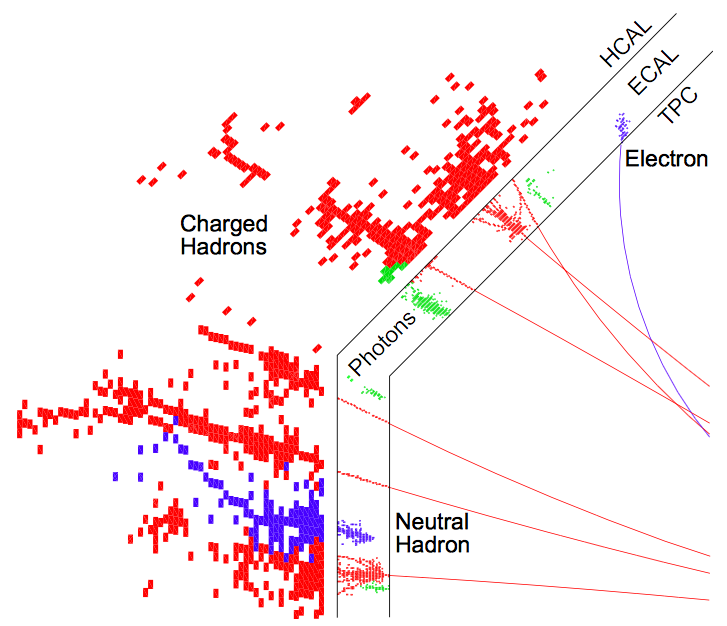
\includegraphics[width=0.5\textwidth]{LCDetectorsAndPFlow/Plots/Pictures/PFlow.png}
\caption[A typical simulated 250 GeV jet in the CLIC\_ILD detector, with labels identifying constituent particles.  Image taken from  \cite{arXiv:1209.4039}.]{A typical simulated 250 GeV jet in the CLIC\_ILD detector, with labels identifying constituent particles.  Image taken from  \cite{arXiv:1209.4039}.}
\label{fig:particleflowpic}
\end{figure} 

%========================================================================================
%========================================================================================

\section{International Large Detector}
\label{sec:ild}
The current detector concepts for the linear collider experiments have been designed to make particle flow calorimetry possible.  While there are a number of different concepts that are under consideration for both the ILC and CLIC, one of the most prominent, and the focus of this work, is the International Large Detector (ILD).  The ILD detector, shown in figure \ref{fig:ild}, achieves very high spatial resolution for all sub-detector systems thanks to its highly segmented calorimeters and central tracking system, both of which are encompassed within a 3.5~T magnetic field.  PandoraPFA \cite{arXiv:1209.4039, arXiv:0907.3577} provides the sophisticated pattern recognition software that is required for particle flow calorimetry.  \textcolor{blue}{A variant of the ILD detector model has also been adapted for use at CLIC and will be discussed in section \ref{sec:clicild}.}

\begin{figure}[h!]
\centering
\subfloat[]{\label{fig:ild1}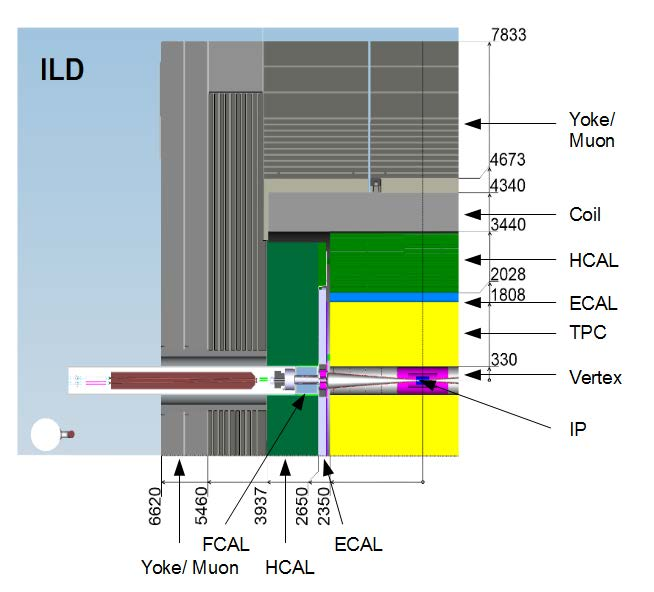
\includegraphics[width=0.5\textwidth]{LCDetectorsAndPFlow/Plots/Pictures/ILD.jpg}}
\subfloat[]{\label{fig:ild2}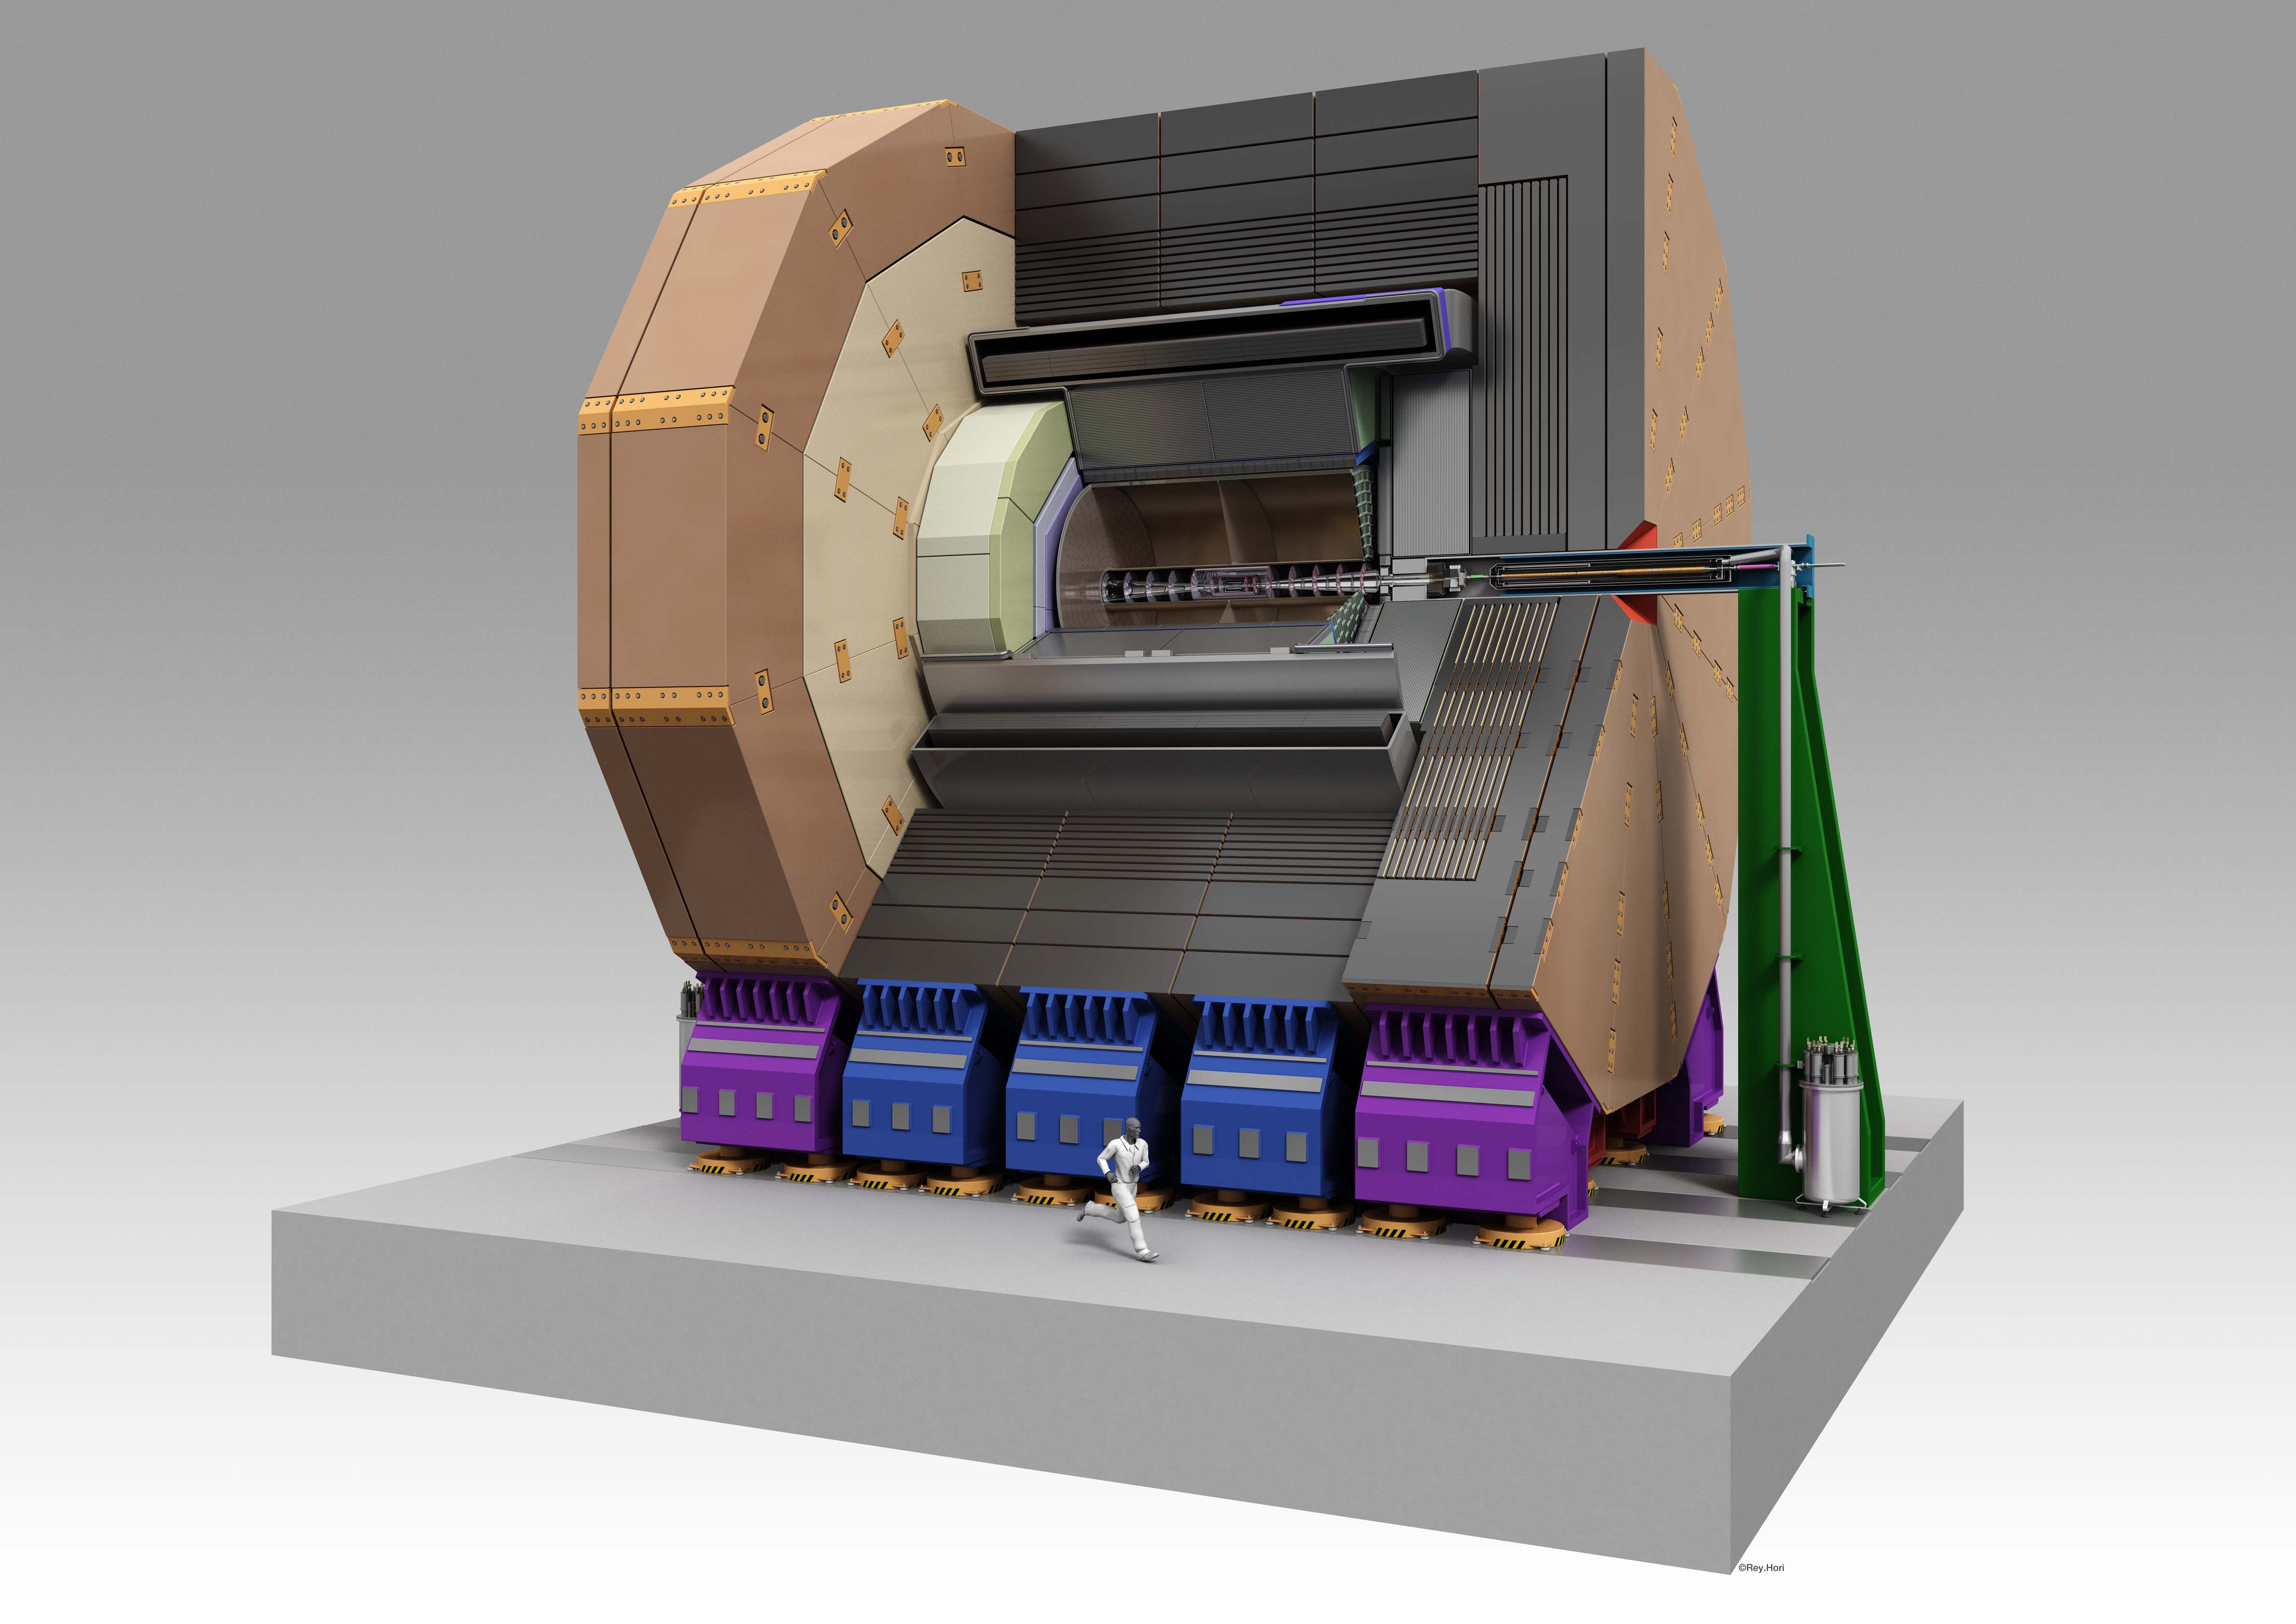
\includegraphics[width=0.5\textwidth]{LCDetectorsAndPFlow/Plots/Pictures/ILD_2.jpg}}
\caption[\protect\subref{fig:ild1} Quadrant view of the ILD detector concept.  The interaction point is in the lower right corner of the picture.  Dimensions are in~mm.  \protect\subref{fig:ild2} An artistic view of the ILD detector concept.  Figures taken from  \cite{Behnke:2013lya}.]{\protect\subref{fig:ild1} Quadrant view of the ILD detector concept.  The interaction point is in the lower right corner of the picture.  Dimensions are in~mm.  \protect\subref{fig:ild2} An artistic view of the ILD detector concept.  Figures taken from  \cite{Behnke:2013lya}.}
\label{fig:ild}
\end{figure} 

%========================================================================================

\subsection{Overview}
The tracking system for the ILD detector consists of a vertex detector, a Time Projection Chamber (TPC) and a number of supplementary silicon detectors.  The vertex detector is designed to give precise information about displaced vertices with respect to the impact point (IP), which is crucial for the study of short lived particles such as the \PD and \PB mesons.  The vertex detector is located close to the IP and surrounding it is the TPC, which is the central tracker for ILD.  The TPC provides detailed measurements of the trajectory of charged particle tracks passing through it, up to 224 measurements per track.  This information is used for determining the curvature of the charged particle track and hence the momentum of the charged particle that traversed it.  Finally, the purpose of the supplementary silicon detectors is to provide additional, high precision, spatial measurements to aid track fitting and extend coverage of the detector down to low polar angles.  

The calorimetric system for the ILD detector is comprised of an electromagnetic calorimeter (ECal), a hadronic calorimeter (HCal) and a number of forward calorimeters (FCal).  The primary function of the ECal is to induce electromagnetic particles to shower within it and to measure the energy of these particle showers.  Similarly, the HCal is designed to induce and measure the energy of hadronic particle showers.  The ECal surrounds the tracking system in the ILD detector and is itself surrounded by the HCal.  The function of FCal is to extend the coverage of the calorimeter system to low polar angles and to provide measurements of the luminosity of the colliding $\text{e}^{\pm}$ beams.  

The outermost elements of the ILD detector are the solenoid, iron yoke and muon system.  The solenoid generates a magnetic field of 3.5~T, which is essential for determining the energy of charged particles in the particle flow paradigm.  The iron yoke is used to return the magnetic field generated by the solenoid.  The yoke is instrumented by the muon system to provide additional information, which supplements the calorimetric energy measurements made by the ILD calorimeters.  

%========================================================================================

\subsection{Vertex Detector}
The main goal of the ILD vertex detector is to achieve a resolution on the impact parameter of charged particle tracks of
\begin{equation}
\sigma_{b} < 5 \oplus \frac{10}{p\text{sin}(\theta)^{3/2}} \text{ {\mu}m,}
\end{equation}
\noindent where $\sigma_{b}$ is the resolution on the track impact parameter, $p$ is the momentum of the track \textcolor{blue}{in units of GeV} and $\theta$ is the angle between the track and the vertex detector plane.  The first term in this parameterisation is the transverse impact parameter\textcolor{blue}{'}s resolution and the second is a multiple-scattering term.  This makes precisely tagging secondary vertices from charm and bottom mesons possible.  Typically these mesons have relatively short proper lifetimes, $\tau$, such that $c\tau \approx \mathcal{O}(300 \text{{ \mu}m})$.  To achieve this impact parameter resolution, a spatial resolution of better than 3~{\mu}m is required near the \textcolor{blue}{interaction} point (IP).  Furthermore, a low material budget of less than 0.15~\% of a radiation length per layer is required to ensure that few electromagnetic showers are initiated within the vertex detector.  A low pixel occupancy is essential for determining the trajectory of individual tracks in the detector.  Furthermore, consideration will have to be given to the mechanical structure of the detector, power consumption and cooling.  

There are a number of different pixel technology options under consideration for the vertex detector for the ILD detector.  This is an active area of ongoing research and development for the linear collider collaboration.  The current design of the vertex detector consists of three concentric layers of double-sided ladders with the first layer containing 10 ladders, the second 11 ladders and the third 17 ladders as shown in figure \ref{fig:vertexpicture}.  Every ladder has two silicon pixel sensors on each side and the ladder thickness is approximately 2~mm.  The radii covered by the detector range from 16~mm to 60~mm from the IP.  \textcolor{blue}{Table \ref{table:vertexdetectorparam} shows the layout, coverage, pitch, spatial resolution and readout times for each of the vertex detector layers.  The first vertex layer is optimised for spatial resolution, while the second layer is optimised for a fast read-out time.  The remaining layers are optimised to reduce power consumption.}  

\begin{table}[h!]
\centering
\begin{tabular}{ l c c c c c c}
\hline
& \multirow{2}{*}{$R$ [mm]} & Coverage & Coverage & Pitch & Spatial & Readout \\
& & [$z$] & [$\text{cos}(\theta)$] & [$\mu\text{m}^{2}$] & Resolution [$\mu$m] & Time [$\mu$s] \\
\hline
Layer 1 & 16 & 62.5 & 0.97 & $17 \times 17$ & 2.8 & 50 \\
Layer 2 & 18 & 62.5 & 0.96 & $17 \times 85$ & 6.0 & 10 \\
\hline
Layer 3 & 37 & 125.0 & 0.96 & $34 \times 34$ & 4.0 & 100 \\
Layer 4 & 39 & 125.0 & 0.95 & $34 \times 34$ & 4.0 & 100 \\
\hline
Layer 5 & 58 & 125.0 & 0.91 & $34 \times 34$ & 4.0 & 100 \\
Layer 6 & 60 & 125.0 & 0.90 & $34 \times 34$ & 4.0 & 100 \\
\hline
\end{tabular}
\caption[Parameters for the ILD vertex detector.  In this table $R$ is the radial position of the vertex layer and $\theta$ is the polar angle with respect to the beam direction.  Table taken from \cite{Behnke:2013lya}.]{\textcolor{blue}{Parameters for the ILD vertex detector.  In this table $R$ is the radial position of the vertex layer and $\theta$ is the polar angle with respect to the beam direction.  Table taken from \cite{Behnke:2013lya}}.}
\label{table:vertexdetectorparam}
\end{table}

\begin{figure}[h!]
\centering
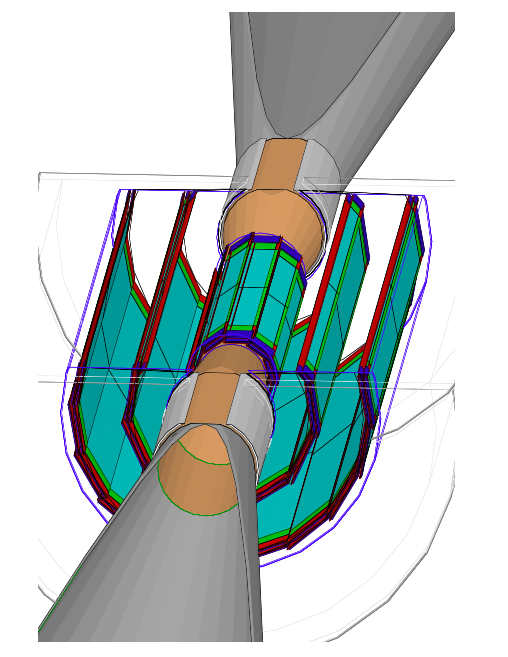
\includegraphics[width=0.3\textwidth]{LCDetectorsAndPFlow/Plots/Pictures/Vertex3.png}
\caption[Vertex detector design for ILD.  Figures taken from \cite{arXiv:1006.3396}.]{Vertex detector design for ILD.  Figures taken from \cite{arXiv:1006.3396}.}
\label{fig:vertexpicture}
\end{figure} 

%========================================================================================

\subsection{Time Projection Chamber}
The central tracking system for the ILD detector is a TPC, which is shown in figure \ref{fig:tracker}.  The TPC consists of a cylindrical gas volume with a central electrode providing an axial electric field.  When a charged particle passes through the TPC, it ionises the gas and the ionised molecules drift in the axial electric field.  The direction of the electric field is chosen such that the electrons drift towards the endplates where they are collected.  The position of the ionisation point can then be calculated using the drift time of the electrons in the TPC.  Combining these TPC hits together makes reconstruction of the charged particle track possible.  TPCs have an advantage over silicon tracking in that they continuously track any charged particle passing through them, while silicon detectors are only sensitive within each silicon layer.  This compensates for the poor single point resolution that TPCs have, \textcolor{blue}{$\sim \mathcal{O}(1 \text{ mm})$}, in comparison to silicon detectors, \textcolor{blue}{$\sim \mathcal{O}(1 \text{ }\mu\text{m})$}, and makes TPCs a viable option for the ILD detector.  Furthermore, TPCs have a very low material budget.  This benefits calorimetry as it minimises energy losses prior to the particle energy entering the calorimeters, which means the calorimetric energy deposits give a better reflection of the true particle energy.  

\textcolor{blue}{In the $xy$ plane} the ILD TPC has a \textcolor{blue}{single} point resolution that is better than 100~{\mu}m and a double hit resolution of $\sim$2~mm\textcolor{blue}{, while in the $xz$ plane the single point resolution is $\sim 1$~mm and the double hit resolution is $\sim 6$~mm.}. The gas used for the TPC will be \textcolor{blue}{Ar:$\text{CH}_4$:$\text{CO}_{2}$} (95:3:2) \cite{arXiv:1006.3396}.  Several readout technology options designed to measure the ionisation current are currently under development.  For all potential options it is envisaged that the readout pads would be $\approx 1 \times 6$~$\text{mm}^{2}$ giving a total of approximately $10^{6}$ pads on each TPC endplate.

\begin{figure}[h!]
\centering
\subfloat[]{\label{fig:tracker1}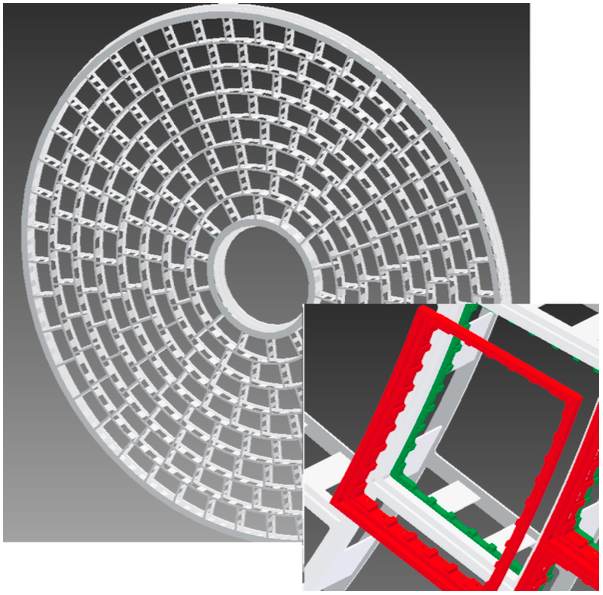
\includegraphics[width=0.5\textwidth]{LCDetectorsAndPFlow/Plots/Pictures/Tracker1.png}}
\subfloat[]{\label{fig:tracker2}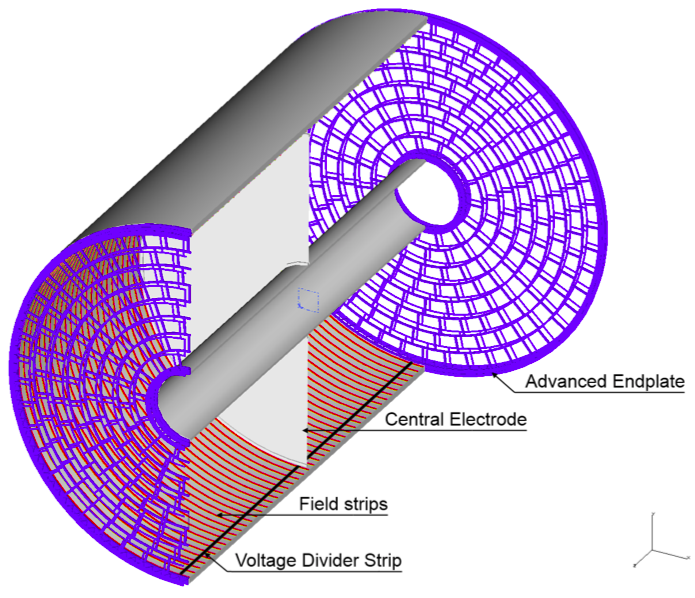
\includegraphics[width=0.5\textwidth]{LCDetectorsAndPFlow/Plots/Pictures/Tracker2.png}}
\caption[\protect\subref{fig:tracker1} Drawing of the proposed end-plate for the TPC.  In the insert a back frame, which is designed to support the readout modules, is shown.  \protect\subref{fig:tracker2} Conceptual sketch of the TPC system showing the main parts of the TPC (not to scale).  The central electrode generates the axial electric field, the endplates collect the ionisation electrons, the field strips help to maintain a uniform electric field across the TPC and the voltage divider strips maintains the voltage difference between the anode and cathode.  The field strips are held at fixed voltages such that they replicate the electric field produced by the electrodes.  This reinforcing of the electric field configuration minimises non-uniformities in the electric field.  The field cage of the TPC is not shown.  Figures taken from  \cite{Behnke:2013lya}\textcolor{blue}{.}]{\protect\subref{fig:tracker1} Drawing of the proposed end-plate for the TPC.  In the insert a back frame, which is designed to support the readout modules, is shown.  \protect\subref{fig:tracker2} Conceptual sketch of the TPC system showing the main parts of the TPC (not to scale).  The central electrode generates the axial electric field, the endplates collect the ionisation electrons, the field strips help to maintain a uniform electric field across the TPC and the voltage divider strips maintains the voltage difference between the anode and cathode.  The field strips are held at fixed voltages such that they replicate the electric field produced by the electrodes.  This reinforcing of the electric field configuration minimises non-uniformities in the electric field.  The field cage of the TPC is not shown.  Figures taken from  \cite{Behnke:2013lya}\textcolor{blue}{.}}
\label{fig:tracker}
\end{figure} 

%========================================================================================

\subsection{Supplemental Silicon Tracking System}
There are four components that make up the supplemental silicon tracking system in the ILD detector, shown in figure \ref{fig:vertex}, which are:
\begin{itemize}
\item Silicon Inner Tracker (SIT) and Silicon External Tracker (SET).  These are both barrel components, which are positioned immediately inside and outside the TPC.  The SIT helps form associations between hits in the vertex detector and the TPC, while the SET helps with extrapolation of TPC tracks into the calorimeter.  
\item Endplate of the TPC (ETD).  This sensor is identical to the SET, but is positioned in front of the ECal endcap calorimeter.  The ETD extends the coverage of the supplemental silicon tracking system envelope. 
\item Forward tracker (FTD).  This detector consists of seven silicon disks that extend the coverage of the tracking down to small angles that are not covered by the TPC.  
\end{itemize}

\begin{figure}[h!]
\centering
\subfloat[]{\label{fig:vertex1}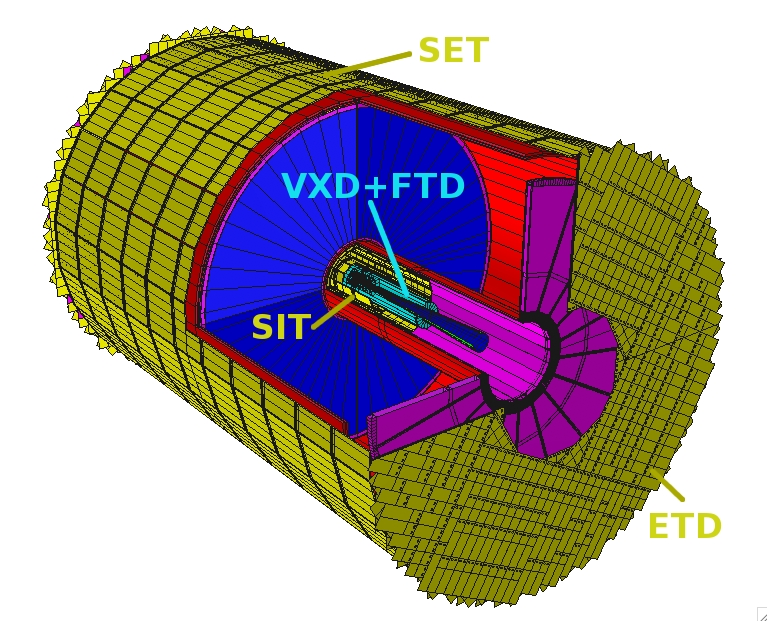
\includegraphics[width=0.5\textwidth]{LCDetectorsAndPFlow/Plots/Pictures/Vertex1.jpg}}
\subfloat[]{\label{fig:vertex2}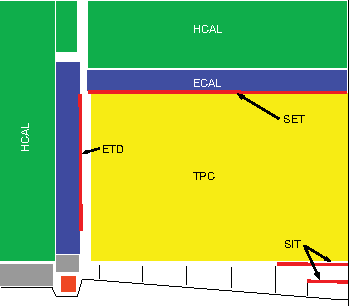
\includegraphics[width=0.5\textwidth]{LCDetectorsAndPFlow/Plots/Pictures/Vertex2.pdf}}
\caption[\protect\subref{fig:vertex1} A 3D detailed GEANT4 simulation description of the silicon system.  \protect\subref{fig:vertex2} A quadrant view of the ILD silicon envelope made of the four components SIT, SET, ETD and FTD as included in the full MOKKA simulation.  Figures taken from  \cite{Behnke:2013lya}.]{\protect\subref{fig:vertex1} A 3D detailed GEANT4 simulation description of the silicon system.  \protect\subref{fig:vertex2} A quadrant view of the ILD silicon envelope made of the four components SIT, SET, ETD and FTD as included in the full MOKKA simulation.  Figures taken from  \cite{Behnke:2013lya}.}
\label{fig:vertex}
\end{figure} 

\begin{table}[h!]
\centering
\begin{tabular}{ l r}
\hline
Tracking System & Coverage [cos($\theta$)] \\
\hline
SIT & 0.910 \\
SET & 0.789 \\
ETD & 0.799 - 0.985 \\
FTD & 0.802 - 0.996\\
\hline
\end{tabular}
\caption[Coverage of the supplementary silicon tracking systems in the ILD detector.  In this table $\theta$ is the polar angle with respect to the beam direction.  Taken from \cite{Behnke:2013lya}.]{Coverage of the supplementary silicon tracking systems in the ILD detector.  In this table $\theta$ is the polar angle with respect to the beam direction.  Taken from \cite{Behnke:2013lya}.}
 \label{table:supptrackingcoverage}
\end{table}

The coverage of the SIT, SET, ETD and FTD is given in table \ref{table:supptrackingcoverage}.  These detectors are designed to give high precision space points that can be used in track fitting.  Furthermore, the ETD and SET are of particular use for extrapolating the charged particle tracks into the calorimeters.  This is key for particle flow calorimetry, which relies upon correct association of charged particle tracks and clusters of calorimeter hits.  Analogously to the vertex detector, these detectors require low material budget and low occupancy.  The FTD, due to its proximity to the beam axis, is particularly prone to high occupancies.  

The SIT, SET and ETD are silicon pixel sensors with 50~{\mu}m pitch embedded in 200~{\mu}m thick silicon.  The FTD consists of seven silicon tracking disks, the first two being pixel detectors and the remaining five being strip detectors.  The pixel detector disks are formed of 16 petals, as shown in figure \ref{fig:ftd}.  Within these petals the pixel size varies from $26 \times 29~{\mu}\text{m}^{2}$ to $26 \times 67~{\mu}\text{m}^{2}$.  Strip detectors are used for the outermost tracking disks as the occupancy considerations do not demand a high granularity detector i.e. a pixel detector.  These detector disks will have a pitch of 50~{\mu}m.  The active sensor and readout ASIC design for each of these detectors is an active area of development for the linear collider.  

\begin{figure}[h!]
\centering
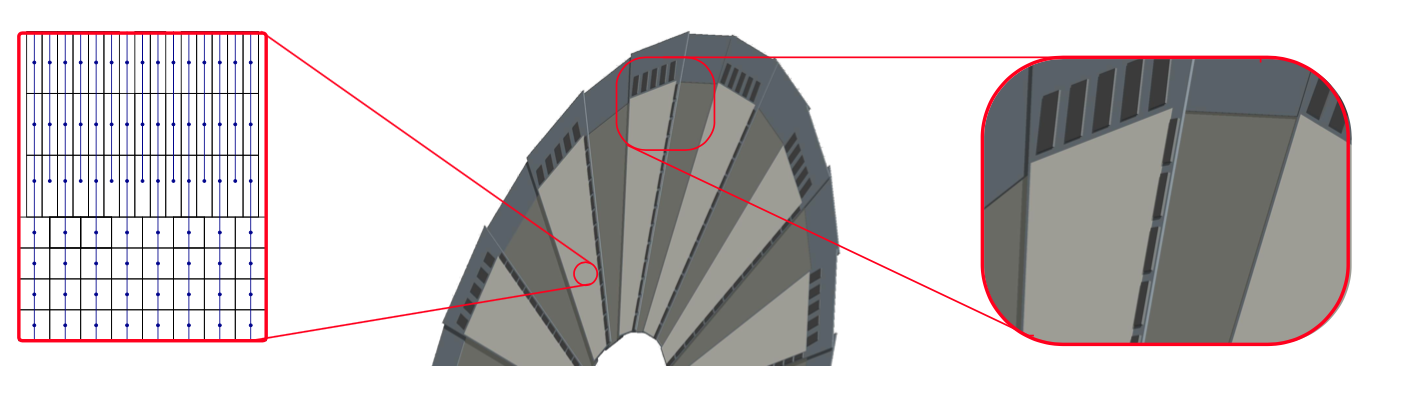
\includegraphics[width=0.8\textwidth]{LCDetectorsAndPFlow/Plots/Pictures/FTD.png}
\caption[A half-disk for the FTD showing the petal concept.  The rightmost zoom image showers a detail of the end-of-petal area that houses the read-out electronics.  The leftmost image shows the region at $R = 8$~cm where both the column width and the $R$-dimension of the pixels changes.  Figures taken from \cite{Behnke:2013lya}.]{A half-disk for the FTD showing the petal concept.  The rightmost zoom image showers a detail of the end-of-petal area that houses the read-out electronics.  The leftmost image shows the region at $R = 8$~cm where both the column width and the $R$-dimension of the pixels changes.  Figures taken from \cite{Behnke:2013lya}.}
\label{fig:ftd}
\end{figure} 

%========================================================================================

\subsection{Electromagnetic Calorimeter}
\label{sec:ildecal}
The nominal ILD detector contains a finely segmented electromagnetic sampling calorimeter (ECal).  The ILD ECal has been specifically designed with particle flow calorimetry in mind.  To that extent the spatial resolution of particle showers within the ECal takes as much, if not more, precedence than the energy resolution.   

There are a number of design requirements for the ECal:
\begin{itemize}
\item The ECal must be compact in size to reduce the overall cost of the detector.
\item Fine segmentation of the ECal is required so that nearby particle showers can be separated.  This is an essential requirement for particle flow calorimetry.
\item Electromagnetic showers should be contained within the ECal.
\end{itemize}
Based on these requirements tungsten is used as the absorber material for the ILD ECal as it has a small radiation length ($X_{0}$), a small \textcolor{blue}{Moli\`{e}re} radius and a large ratio of radiation length to nuclear interaction length.  A comparison of these properties for other ECal absorber material candidates is shown in table \ref{table:absorberoptions}.  The small radiation length in tungsten allows for a large number of radiation lengths, $\approx 24$~$X_{0}$, to be compacted within a relatively short distance, $\approx 20$~cm, in the nominal ILD ECal.  This is sufficient for containing all but the highest energy electromagnetic showers.  The small \textcolor{blue}{Moli\`{e}re} radius in tungsten will lead to compact electromagnetic showers.  This makes separation of nearby showers easier.  Finally, the large ratio of the radiation length to the nuclear interaction length in tungsten will lead to greater longitudinal separation between electromagnetic and hadronic showers, again making shower identification easier.   

\begin{table}[h!]
\centering
\begin{tabular}{ l l l l l}
\hline
Material & $\lambda_{I}$ [cm] & $X_{0}$ [cm] & $\rho_{M}$ [cm] & $ \lambda_{I}/X_{0}$ \\
\hline
Fe & 16.8 & 1.76 & 1.69 & 9.5 \\
Cu & 15.1 & 1.43 & 1.52 & 10.6 \\
W & 9.6 & 0.35 & 0.93 & 27.4 \\
Pb & 17.1 & 0.56 & 1.00 & 30.5 \\
\hline
\end{tabular}
\caption[Comparison of the nuclear interaction length $\lambda_{I}$, radiation length $X_{0}$ and \textcolor{blue}{Moli\`{e}re} radius for iron, copper, tungsten and lead.  Table taken from \cite{arXiv:0907.3577}.]{Comparison of the nuclear interaction length $\lambda_{I}$, radiation length $X_{0}$ and \textcolor{blue}{Moli\`{e}re} radius for iron, copper, tungsten and lead.  Table taken from \cite{arXiv:0907.3577}.}
\label{table:absorberoptions}
\end{table}

The active material in the nominal ILD ECal is silicon, however, a scintillator strip option is also being considered.  Figure \ref{fig:ecalimage} shows a cross section through a layer of the ECal for both of these options.  It contains a total of 30 longitudinal readout layers, which is sufficient to provide a good energy resolution.  The tungsten thickness for the innermost 20 layers is 2.1~mm, while for the final 10 layers it is 4.2~mm.  This configuration of absorber material thickness is chosen to reduce the number of readout channels and hence the cost, while maintaining a high sampling rate for particle showers at the start of the ECal.  It should be noted that this ECal offers no gains in terms of energy resolutions in comparison to pre-existing particle collider experiments, as shown in table \ref{table:ecalenergyres}.  This is the case because the focus of this calorimeter is split between imaging the particle showers and recording their energy as opposed to purely focusing on the energy measurement.  Each of the ECal layers is divided up into square cells, of 5~mm side length, which makes separation of nearby particle showers possible.  This cell size was chosen as a balance between being able to resolve nearby particle showers and reducing the overall cost of the calorimeter, which scales with the number of readout channels.  An optimisation study of the various ECal parameters for the ILD detector can be found in section \ref{sec:ecal}.

\begin{figure}[h!]
\centering
\subfloat[]{\label{fig:ecalimage1}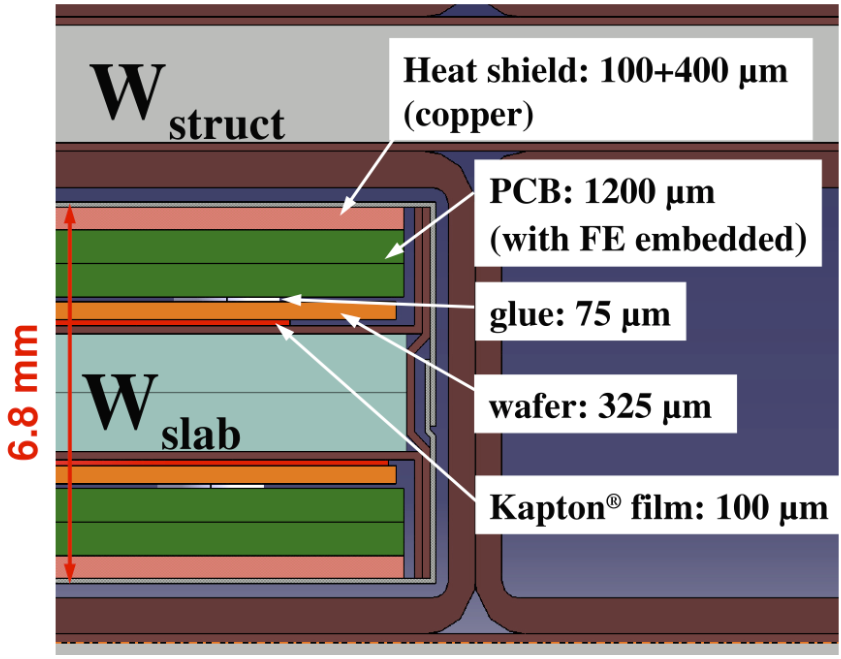
\includegraphics[width=0.4\textwidth]{LCDetectorsAndPFlow/Plots/Pictures/SiECal.png}} 
\hspace{1cm}
\subfloat[]{\label{fig:ecalimage2}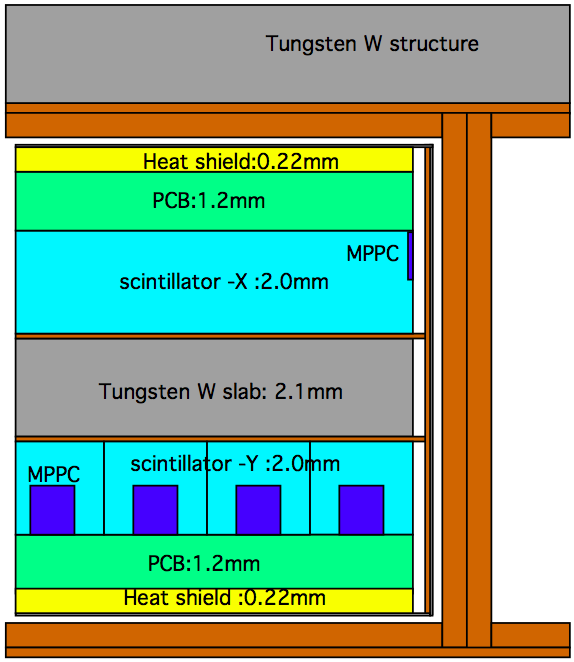
\includegraphics[width=0.4\textwidth]{LCDetectorsAndPFlow/Plots/Pictures/ScECal.png}}
\caption[Cross section through \textcolor{blue}{an} ECal layer for \textcolor{blue}{the} \protect\subref{fig:ecalimage1} silicon and \protect\subref{fig:ecalimage2} scintillator options.  Figures taken from  \cite{Behnke:2013lya}.]{Cross section through \textcolor{blue}{an} ECal layer for \textcolor{blue}{the} \protect\subref{fig:ecalimage1} silicon and \protect\subref{fig:ecalimage2} scintillator options.  Figures taken from  \cite{Behnke:2013lya}.}
\label{fig:ecalimage}
\end{figure} 

\begin{table}[h!]
\centering
\begin{tabular}{ l l }
\hline
Experiment & ECal Energy Resolution $\frac{\sigma_{E}}{E}$ \\
\hline
CMS \cite{Chatrchyan:2013dga} & $\sim \frac{2.8\%}{\sqrt{E(\text{GeV})}} \oplus 0.3\% \oplus \frac{12\%}{E(\text{GeV})}$ \\
ATLAS \cite{Aharrouche:2006nf} & $\sim \frac{10.1\%}{\sqrt{E(\text{GeV})}} \oplus 0.1\%$ \\
LHCb \cite{Perret:2014owa} & $\sim \frac{9\%}{\sqrt{E(\text{GeV})}} \oplus 0.8\%$ \\
\textcolor{blue}{OPAL} \cite{Ahmet:1990eg} & $\sim \frac{6.3\%}{\sqrt{E(\text{GeV})}}$ \\
\textcolor{blue}{ALEPH} \cite{Buskulic:1994wz} & $\sim \frac{17.9\%}{\sqrt{E(\text{GeV})}} \oplus 1.9\%$ \\
ILC (ILD Silicon Option) \cite{Behnke:2013lya} & $\sim \frac{16.6\%}{\sqrt{E(\text{GeV})}} \oplus 1.1\%$ \\
\hline
\end{tabular}
\caption[Comparison of the ECal energy resolutions for various experiments.]{Comparison of the ECal energy resolutions for various experiments.}
\label{table:ecalenergyres}
\end{table}

%========================================================================================

\subsection{Hadronic Calorimeter}
A finely segmented hadronic sampling calorimeter (HCal) is used in the nominal ILD detector.  The design requirements for the ILD HCal mirror those of the ECal, which can be found in section \ref{sec:ildecal}, with one exception; the HCal is designed to contain hadronic showers as opposed to electromagnetic showers.  Steel is used as the absorber material for the HCal as it has durable mechanical properties that allow the HCal to be constructed without the need for auxiliary supports.  When required, auxiliary supports create dead regions in the detector that would harm performance.  Furthermore, steel is relatively inexpensive and has a small nuclear interaction length, meaning it is possible to achieve a compact calorimeter design at low cost.  The nominal ILD HCal contains approximately $6 \lambda_{I}$, which when combined with the $1 \lambda_{I}$ in the ECal is enough to contain the majority of hadronic showers at ILC like energies.  

The active material in the nominal ILD HCal is scintillator.  In total, the HCal contains 48 readout layers, which provides an extremely good energy resolution.  This can be seen when comparing the HCal energy resolution between different experiments, as shown in table \ref{table:hcalenergyres}.  An individual layer in the HCal is comprised of 20~mm of steel absorber material with 3~mm of scintillator active material.  Each layer in the HCal is segmented into square cells of side length 30~mm.  This cell size was chosen as a balance between reducing the cost of the detector, which is proportional to the number of readout channels, and achieving the required spatial resolution to make particle flow calorimetry possible.  The segmentation of the ILD HCal gives excellent spatial resolution and sufficiently good energy resolution to make the use of particle flow calorimetry a reality.  An optimisation study of the various HCal parameters for the ILD detector can be found in section \ref{sec:hcal}.

The ILD HCal is intrinsically non-compensating, which means that it has a different response to electromagnetic and hadronic showers.  The origin of this different response is the fundamentally different mechanisms governing the propagation of electromagnetic and hadronic showers.  One key difference between the mechanisms is that hadronic showers have an invisible energy component, which occurs due to  effects such as neutrons coming to rest in the detector and nuclear \textcolor{blue}{binding} energy losses \cite{Tran:2017tgr}.  In general, this leads to a lower response from a calorimeter to a hadronic shower than an electromagnetic shower.  A number of different software techniques have been developed for the linear collider experiment that attempt to correct this non-compensating response.  For more details see chapter \ref{chap:energyestimators}.  The ILD ECal has a compensating response due to the use of tungsten as the absorber material \cite{Blaising:2015nla}, therefore, no additional treatment of energies is required.

\begin{table}[h!]
\centering
\begin{tabular}{ l l }
\hline
Experiment & HCal Energy Resolution $\frac{\sigma_{E}}{E}$ \\
\hline
CMS \cite{Budd:2001eu} & $\sim \frac{90\%}{\sqrt{E(\text{GeV})}} \oplus 4.8\%$ \\
ATLAS \cite{Airapetian:1996iv} & $\sim \frac{52.1\%}{\sqrt{E(\text{GeV})}} \oplus 3.0\% \oplus \frac{1.6\%}{E(\text{GeV})}$ \\
LHCb \cite{Perret:2014owa} & $\sim \frac{69\%}{\sqrt{E(\text{GeV})}} \oplus 9.0\%$ \\
\textcolor{blue}{OPAL} \cite{Ahmet:1990eg} & $\sim \frac{120\%}{\sqrt{E(\text{GeV})}}$ \\
\textcolor{blue}{ALEPH} \cite{Buskulic:1994wz} & $\sim \frac{85\%}{\sqrt{E(\text{GeV})}}$ \\
ILC (ILD Silicon Option) \cite{Behnke:2013lya} & $\sim \frac{43.3\%}{\sqrt{E(\text{GeV})}} \oplus 1.8\%$ \\
\hline
\end{tabular}
\caption[Comparison of the HCal energy resolutions for various experiments.]{Comparison of the HCal energy resolutions for various experiments.}
\label{table:hcalenergyres}
\end{table}

%========================================================================================

\subsection{Solenoid, Yoke and Muon System}
Surrounding the ILD calorimeter system is the solenoid that generates a 3.5~T magnetic field.  The magnetic field produced by the coil is crucial for bending charged particles so that their momentum can be determined from the curvature of the path they traverse.  Furthermore, the bending of charged particles leads to greater separation of calorimetric energy deposits between charged and neutral particles, which will reduce the effects of confusion when using particle flow calorimetry.  

The magnetic field in the ILD detector is returned by an iron yoke that surrounds the solenoid.  Iron is chosen for the yoke material as it has a very large permeability.  The yoke is instrumented by a muon system in the barrel and forward regions of the detector.  The goal of this instrumentation is to identify muons escaping the calorimeters and to act as a tail catcher for the calorimeters.  The muon system consists of 10 layers, spaced 140~mm apart, followed by 2 and 3 layers spaced 600~mm apart in the barrel and endcap regions of the detector respectively, as shown in figure \ref{fig:muon}.  There is also an additional sensitive layer for the barrel region placed immediately outside the HCal to help with association energy deposits between the calorimeters and the yoke.  As the majority of particles at ILC like energies will be contained within the calorimeters, the energy and spatial resolution of the muon system are not critical to performance.  It is for that reason that the number of layers is lower and the layer thicknesses wider in the yoke than in the calorimeters.  The nominal ILD model uses 30~mm wide and 1 m long scintillator strips as the readout technology for the yoke.

\begin{figure}[h!]
\centering
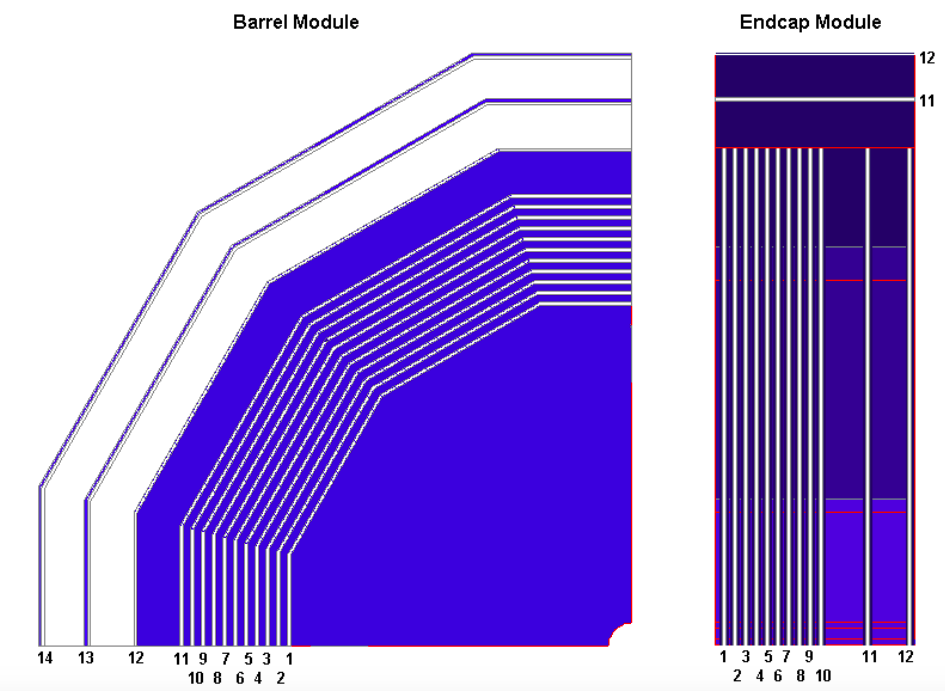
\includegraphics[width=0.5\textwidth]{LCDetectorsAndPFlow/Plots/Pictures/Muon.png}
\caption[The sensitive layers of the ILD muon system.  Figure taken from  \cite{Behnke:2013lya}.]{The sensitive layers of the ILD muon system.  Figure taken from  \cite{Behnke:2013lya}.}
\label{fig:muon}
\end{figure}   

%========================================================================================

\subsection{Forward Calorimetry}
Forward calorimetry in the ILD detector consists of three additional sampling calorimeters:
\begin{itemize}
\item The LumiCal, which is located within the octagonal hole in the ECal endcap.  This will give a precise measurement of the luminosity of the linear collider beam.   The LumiCal uses Bhabha scattering, $\text{e}^{+}\text{e}^{-} \rightarrow \text{e}^{+}\text{e}^{-}(\gamma)$, as a gauge process for the luminosity measurement.  Using this approach the luminosity can be measured with precision of less than $10^{-3}$ at $\sqrt{s}=500$~GeV \cite{arXiv:1006.3396}. 
\item The LHCal, which is positioned within the square hole of the HCal endcap.  This hadronic calorimeter is designed to extend the coverage of the HCal down to small polar angles.  
\item The BeamCal, which is located just in front of the final focusing quadrupole.  This calorimeter will perform a bunch-by-bunch estimate of the luminosity based on the energy deposited in the calorimeter.
\end{itemize}
The layout of these calorimeters is shown in figure \ref{fig:fcal} and their coverage is summarised in table \ref{table:fcalcoverage}.  Each of the forward calorimeters will have to deal with high occupancies due to the presence of background processes, e.g. beamstrahlung, which makes fast readout crucial.  Furthermore, the BeamCal experiences a large flux of low energy electrons due to its proximity to the beam pipe, which results in a large radiation dose.  This makes radiation hard sensors essential for the BeamCal.  

\begin{figure}[h!]
\centering
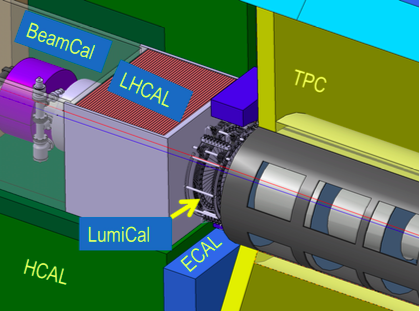
\includegraphics[width=0.5\textwidth]{LCDetectorsAndPFlow/Plots/Pictures/FCal.png}
\caption[The very forward region of the ILD detector.  LumiCal, BeamCal and LHCal are carried by the support tube for the final focusing quadruple, QD0, and the beam pipe.  Figure taken from  \cite{Behnke:2013lya}.]{The very forward region of the ILD detector.  LumiCal, BeamCal and LHCal are carried by the support tube for the final focusing quadruple, QD0, and the beam pipe.  Figure taken from  \cite{Behnke:2013lya}.}
\label{fig:fcal}
\end{figure} 

\begin{table}[h!]
\centering
\begin{tabular}{ l r }
\hline
Forward Calorimeter & Polar Angle Coverage [mrad] \\
\hline
LumiCal & $31 - 77$ \\
LHCal & $\sim 29 - 122$ \\
BeamCal & $5 - 40$ \\
\hline
\end{tabular}
\caption[Coverage of the forward calorimeters in the ILD detector.]{Coverage of the forward calorimeters in the ILD detector.}
\label{table:fcalcoverage}
\end{table}

Each of these forward calorimeters is constructed using tungsten as the absorber material.  The small \textcolor{blue}{Moli\`{e}re} radius of tungsten ensures that narrow electromagnetic showers are formed within them, which makes separation and identification of showering particles easier.  

The layout of these calorimeters is as follows:
\begin{itemize}
\item The LumiCal is a silicon tungsten sampling calorimeter that contains 30 readout layers.  This gives the LumiCal a total depth of $\approx 24 X_{0}$.  
\item The LHCal is also a silicon tungsten sampling calorimeter, which contains 40 readout layers.  The total depth of the LHCal is $\approx 4 \lambda_{I}$.
\item The BeamCal is a tungsten based sampling calorimeter.  The sensitive detector material for the BeamCal is an ongoing area of research as, due to the extremely high occupancy from the beam induced backgrounds, a very fast readout is required.  The exact layer configuration of the BeamCal will depend upon the choice of sensitive detector material and hence is yet to be specified.  
\end{itemize}
The segmentation within the layers, i.e. the cell size, in these forward calorimeters is yet to be fully optimised.

%========================================================================================

\section{Simulation}
\label{sec:simulation}
Detector model simulation for all studies presented in this work was performed using MOKKA \cite{MoradeFreitas:2002kj}, a GEANT4 \cite{Agostinelli:2002hh,Allison:2006ve} wrapper providing detailed geometric descriptions of detector concepts for the linear collider.  The MOKKA simulation of the ILD detector includes the following \cite{Behnke:2013lya}:
\begin{itemize}
\item The vertex detector is simulated using silicon as the sensitive material.  Support material and the cryostat are also included.
\item The supplementary silicon tracking systems are included.  Again, material has been added to the simulation to represent the support material for these systems.  Furthermore, an estimation has been made of the material budget for power and readout cables from the vertex detector, SIT and FTD and material has been added to the simulation to represent these.  The material added to represent the power and readout cables comes in the form of an aluminium cylinder running inside the TPC field cage and a cone around the beam pipe.
\item The TPC is simulated as a cylindrical volume of a gas mixture surrounded by a field cage.  A conservative estimate of the endplate is included in the simulation to account for the support structure, electronics and cooling pipes for the TPC.
\item As well as including the silicon tungsten sampling calorimeter, the simulation of the ILD ECal contains additional material to represent the instrumented region of the sensor and a heat shield as shown in figure \ref{fig:ecalimage}.
\item Simulation of the ILD HCal has a number of realistic features including detailed modelling of the electronics, detector gaps and the implementation of Birk's law \cite{Birks:1951boa} for the scintillator sensitive detector elements.  \textcolor{blue}{Birk's law accounts for the non linear relationship between the energy deposited per unit length and the amount of scintillation light produced when a charged particle passing through a scintillator.}
\item The muon system, which is the instrumentation of the iron yoke, uses scintillator as the active material in the simulation.  A square cell size of side length 30~mm is assumed.  This is in contrast to the nominal ILD model, but as the tail-catcher plays a minimal role in event reconstruction at ILC like energies this difference should have negligible impact.  
\item The forward calorimeters, the LumiCal, LHCal and BeamCal, are all included in the simulation.  Tungsten is used as the absorber material for each of the calorimeters.  The LumiCal and LHCal use a silicon readout material, while the BeamCal uses a diamond readout.  
\end{itemize}

The simulation and reconstruction of the large event samples used in the studies presented in the work was performed using the ILCDIRAC \cite{Grefe:2014sca, Tsaregorodtsev:2008zz} grid production tools.  

%========================================================================================

\section{CLIC\_ILD}
\label{sec:clicild}
The increased collision energy of the proposed CLIC accelerator means the use of the nominal ILD detector model would be inappropriate.  Therefore, a new detector model, CLIC\_ILD \cite{Linssen:2012hp,AlipourTehrani:2254048}, based upon the nominal ILD detector model was created to cope with the experimental conditions found at the CLIC experiment.  \textcolor{blue}{Figure \ref{fig:clicild} shows the longitudinal and transverse cross sections of the CLIC\_ILD detector.}  The main differences between the nominal ILD detector and CLIC\_ILD are:

\begin{figure}[h!]
\centering
\subfloat[]{\label{fig:clicild1}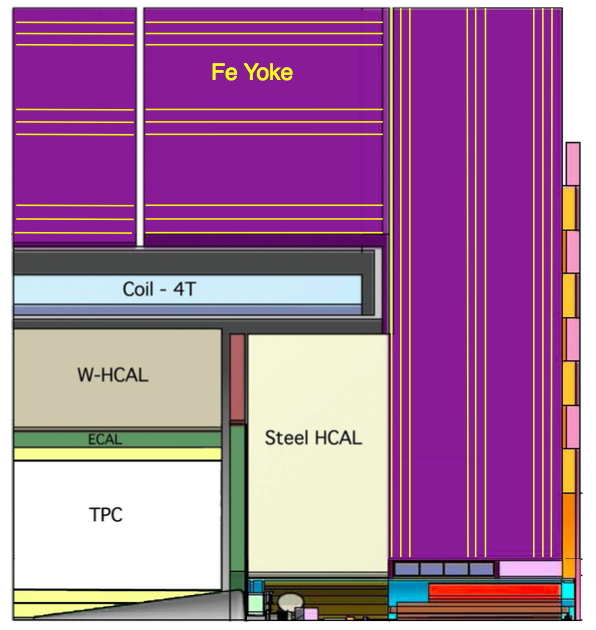
\includegraphics[width=0.4\textwidth]{LCDetectorsAndPFlow/Plots/Pictures/CLIC_ILD.png}}
\hspace{1cm}
\subfloat[]{\label{fig:clicild2}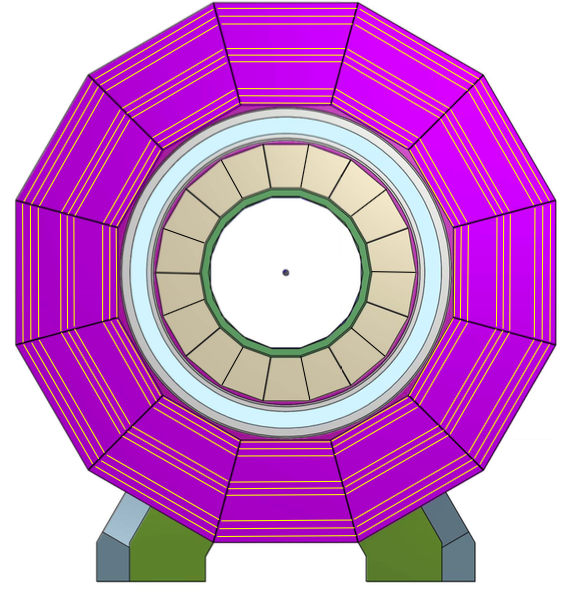
\includegraphics[width=0.4\textwidth]{LCDetectorsAndPFlow/Plots/Pictures/CLIC_ILD_2.png}}
\caption[\protect\subref{fig:ild1} Longitudinal (top quadrant) and \protect\subref{fig:ild2} transverse cross section of the CLIC\_ILD detector.  Figures taken from \cite{Linssen:2012hp}.]{\protect\subref{fig:ild1} Longitudinal (top quadrant) and \protect\subref{fig:ild2} transverse cross section of the CLIC\_ILD detector.  Figures taken from \cite{Linssen:2012hp}.}
\label{fig:clicild}
\end{figure} 

\begin{itemize}
\item The higher energies found at the CLIC experiment lead to more intense beam induced backgrounds, which is especially problematic for detectors close to the IP where the occupancies will be extremely high.  For this reason the inner vertex detector in CLIC\_ILD is moved 15~mm further out from the IP.    
\item The HCal thickness is increased from 6 $\lambda_{I}$ to 7.5 $\lambda_{I}$.  This ensures that higher energy hadronic showers found at the CLIC experiment are contained within the calorimeters.  
\item The HCal absorber material for the barrel is tungsten as opposed to steel.  This reduces the overall thickness of the HCal and keeps the coil size, one of the driving cost factors for the detectors, similar for the nominal ILD and CLIC\_ILD detectors.  Steel is used as the absorber material for the HCal endcaps as there are no spatial requirements relating to the coil size and this will lower the detector cost.  Furthermore, the shower development time in steel is faster than in tungsten.  This makes effective time stamping of energy deposits easier, which is crucial for the CLIC experiment for vetoing beam induced backgrounds.  
\item The magnetic field strength in the CLIC\_ILD detector is increased to 4 T.  This was found to benefit the reconstruction, particularly at high energies, as it leads to greater separation of charged particle tracks.  Furthermore, it was possible to achieve this increase in field strength using the nominal ILD coil design.   
\item The CLIC\_ILD detector contains masking, graphite layers placed in front of the BeamCal, to prevent particles produced by the beam-induced interactions from backscattering into the main detector.  It is the increased collision energy that makes backscattering of particles a more problematic effect for the CLIC experiment than it is for the ILC experiment.   
\end{itemize}  

The CLIC\_ILD detector will be used for the study of anomalous gauge couplings presented in chapter \ref{chap:PhysicsAnalysis}.

%========================================================================================
%======================================================================================== 

\section{Particle Flow Reconstruction}
\label{sec:reconstruction}
Particle flow calorimetry relies upon correct associations being made between calorimetric energy deposits and charged particle tracks.  Even with a finely segmented detector, such as the ILD detector described in section \ref{sec:ild}, correctly making these associations is a highly non-trivial task and must be done using advanced pattern recognition software.  This is provided by the PandoraPFA particle flow algorithm \cite{Marshall:2015rfa}.  PandoraPFA is applied in the linear collider reconstruction using MARLIN \cite{Gaede:2006pj}, a c++ framework specifically designed for the linear collider.  

%======================================================================================== 

\subsection{PandoraPFA}
PandoraPFA's inputs are calorimeter hits and charged particles tracks and it produces as output reconstructed particles known as particle flow objects (PFOs).  The pattern recognition in PandoraPFA is applied in eight main stages as described in the original PandoraPFA paper \cite{arXiv:0907.3577} and the CLIC focused PandoraPFA paper \cite{arXiv:1209.4039}:
\begin{enumerate}
\item Track selection.  The input track collections are examined to determine whether $V^{0}$ decays or kinks are present.  Two charged tracks originating from a point displaced from the IP indicates the presence of a $V^{0}$ decay.  \textcolor{blue}{The vertex of any $V^{0}$ decay is required to be at least 5~mm from the IP.  The $V^{0}$ decays that PandoraPFA attempts to identify are $\gamma \rightarrow \text{e}^{+}\text{e}^{-}$, $K^{0}_{S} \rightarrow \pi^{+}\pi^{-}$, $\Lambda \rightarrow \text{p}\pi^{-}$ and $\bar{\Lambda} \rightarrow \bar{\text{p}}\pi^{+}$.  These decays are distinguished from each other by performing a mass hypothesis test using the charge and momenta of the tracks identified as coming from a $V^{0}$ decay.} A charged particle decaying into a single charged particle and a number of neutral ones indicates a kink.  The $V^{0}$ decay and kink information will be propagated in the reconstruction to the final PFO creation stage.  
\item Calorimeter hit treatment.  The treatment of calorimeter hits by PandoraPFA is of paramount importance to the work presented in chapters \ref{chap:energyestimators} and \ref{chap:detopt}.  Therefore, full details of the calorimeter hit selection procedure are presented here.  This selection procedure is broken down into several steps:
\begin{itemize}
\item The various collection\textcolor{blue}{s} of, post digitisation, calorimeter hits are passed into the Pandora framework and converted into Pandora calorimeter hits.  
\item To minimise any \textcolor{blue}{dependency} on the detector geometry each calorimeter hit is assigned to a pseudo-layer\textcolor{blue}{, which is illustrated in figure \ref{fig:pseudolayer}.  Pseudo-layers are defined using the amount of material found between any given point in the calorimeters and the IP.  This makes them the natural construct for parameterising particle shower development along the direction of travel of showering particles.  Therefore, all further topological association algorithms in PandoraPFA work using the pseudo-layer definition.}
\item A minimum ionising particle \textcolor{blue}{MIP} equivalent energy cut is applied to the calorimeter hits.  If a calorimeter hit contains less than 0.5 (0.3) of the energy of a normally incident MIP passing through the calorimeter cell in the ECal (HCal) then it is not used in the reconstruction.  
\item If a calorimeter hit is sufficiently far away from other hits it is flagged as an isolated hit.  Such hits are most likely due to low energy neutrons produced in hadronic showers \textcolor{blue}{that} can travel a significant distance from the original shower before depositing energy.  Due to the distance they travel, these hits are very difficult to associate to the correct particle shower.  Furthermore, as such hits are unlikely to be the seed for a particle shower, they are not used by the initial clustering algorithm.  
\item Any calorimeter hit that contains an energy consistent with a MIP signal and where one Pandora calorimeter hit at most exists in the neighbouring \textcolor{blue}{cells} within the same layer is flagged as a MIP consistent hit.  This information is used in the identification of MIPs in the reconstruction.
\item The energy contribution for each calorimeter hit ultimately depends on whether the cluster the calorimeter hit has been associated to is deemed to have originated from an electromagnetic or hadronic particle shower.  Different scale factors are applied to the energy for electromagnetic and hadronic showers to account for the non-compensating response of the calorimeters.  These scale factors are used throughout the reconstruction, including the final reconstructed particle energy, once the particle shower type has been identified.  For energy comparisons prior to the shower type being identified, the uncorrected calorimeter hit energy is used.  Further details on how these calibration constants are determined can be found in chapter \ref{chap:energyestimators}.  
\end{itemize}
\item Clustering.  This begins by using the projection of the charged particle tracks onto the front face of the ECal as seeds for the initial clustering phase.  Calorimeter hits are looped over on a per layer basis, working from the inner to the outer pseudo-layer, and if they fall within a cone of fixed dimensions surrounding a cluster direction they are associated to the cluster.  If no association can be made to any pre-existing calorimeter hit clusters then the calorimeter hit is used to seed a new cluster.  
\item Topological cluster merging.  The initial clustering algorithm is designed to be conservative to avoid mixing together energy deposits from several particles.  The fragments produced by the initial clustering are then merged together by various algorithms whose logic is determined by a number of well-motivated topological rules, such as those shown figure \ref{fig:associations}.  
\item Statistical re-clustering.  Comparisons between the cluster energy and any associated track momenta are made to determine whether they are consistent.  
\textcolor{blue}{A consistent track-cluster match is defined by the magnitude of the difference between the track momenta, $p_{Track}$, and cluster energy being less than three $\sigma$, where $\sigma = 60\% \times p_{Track}$, which is the approximate hadronic energy resolution of the ILD calorimeters.}  If a large discrepancy is observed then statistical re-clustering is initiated.  This involves running a number of differently configured algorithms to change the cluster configuration to determine if a new optimal configuration of tracks and clusters can be found.  

This step relies upon the reported cluster energies being accurate.  To ensure this is the case, a well defined calibration procedure is applied for all detector models considered in this work, for more details see chapter \ref{chap:energyestimators}.  At this point in the reconstruction, the energy resolution of the calorimeters impacts the way that the pattern recognition is performed.  The better the energy resolution of the calorimeters, the fewer the number of mistakes that are made when pairing up clusters of calorimeter hits to charged particle tracks.    

\item Photon identification and recovery.  Topological likelihood data is used to identify clusters of calorimeter hits that are consistent with photons.  This is possible due to the clear transverse and longitudinal profiles observed for electromagnetic showers.  
\item Fragment removal.  Neutral clusters originating from a nearby charged particle cluster are identified and merged back into the parent charged particle cluster.  These algorithms take into account the changes in the compatibility of the track and cluster associations when merging any neutral clusters into charged clusters.  
\item Formation of particle flow objects.  Finally, reconstructed particles are produced.  The energy for charged particles is taken from the track momenta, while neutral particle energies are taken from the calorimeter cluster measurements.  Furthermore, the different electromagnetic and hadronic scales are applied to the output neutral particle energies depending on whether the neutral cluster is consistent with a photon.  
\end{enumerate}

\begin{figure}[h!]
\centering
\subfloat[]{\label{fig:pseudolayer1}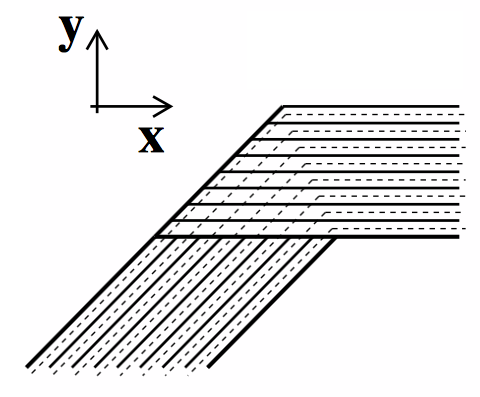
\includegraphics[width=0.4\textwidth]{LCDetectorsAndPFlow/Plots/Pictures/PseudoLayer1.png}}
\hspace{1cm}
\subfloat[]{\label{fig:pseudolayer2}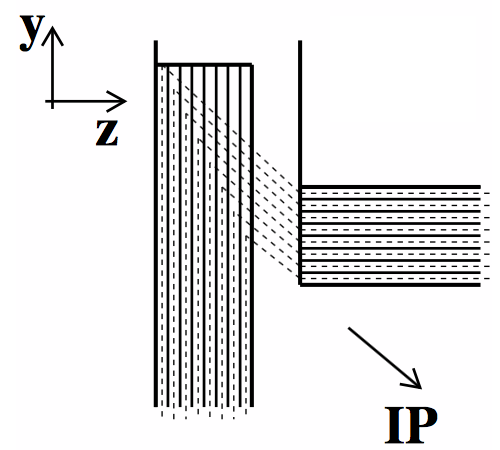
\includegraphics[width=0.4\textwidth]{LCDetectorsAndPFlow/Plots/Pictures/PseudoLayer2.png}}
\caption[Schematic showing the definition of the pseudo-layer assignment for calorimeter hits.  The solid lines indicate the positions of the physics ECal layers and the dashed lines show the definition of the virtual pseudo-layers.  \protect\subref{fig:pseudolayer1} The $xy$-view shows the ILD ECal stave structure.  \protect\subref{fig:pseudolayer2} The $xz$ view shows a possible layout for the ECal barrel/endcap overlap region.  The pseudo-layers are defined using projection back to the IP.  Figures taken from \cite{arXiv:0907.3577}.]{Schematic showing the definition of the pseudo-layer assignment for calorimeter hits.  The solid lines indicate the positions of the physics ECal layers and the dashed lines show the definition of the virtual pseudo-layers.  \protect\subref{fig:pseudolayer1} The $xy$-view shows the ILD ECal stave structure.  \protect\subref{fig:pseudolayer2} The $xz$ view shows a possible layout for the ECal barrel/endcap overlap region.  The pseudo-layers are defined using projection back to the IP.  Figures taken from \cite{arXiv:0907.3577}.}
\label{fig:pseudolayer}
\end{figure} 

\begin{figure}[h!]
\centering
\subfloat[]{\label{fig:association1}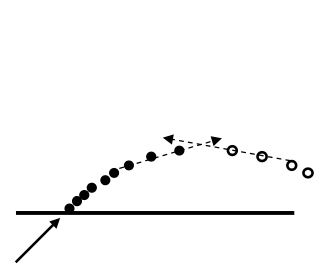
\includegraphics[width=0.2\textwidth]{LCDetectorsAndPFlow/Plots/Pictures/Association1.png}}
\hspace{5mm}
\subfloat[]{\label{fig:association2}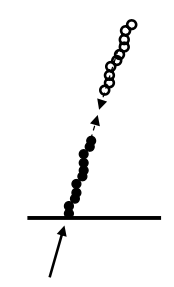
\includegraphics[width=0.2\textwidth]{LCDetectorsAndPFlow/Plots/Pictures/Association2.png}}
\hspace{5mm}
\subfloat[]{\label{fig:association3}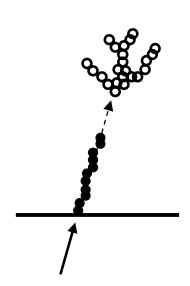
\includegraphics[width=0.2\textwidth]{LCDetectorsAndPFlow/Plots/Pictures/Association3.png}}
\hspace{5mm}
\subfloat[]{\label{fig:association4}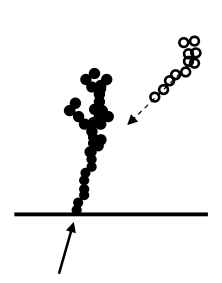
\includegraphics[width=0.2\textwidth]{LCDetectorsAndPFlow/Plots/Pictures/Association4.png}} \\
\subfloat[]{\label{fig:association5}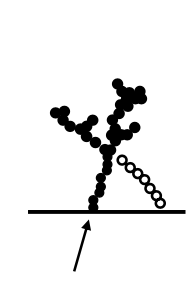
\includegraphics[width=0.2\textwidth]{LCDetectorsAndPFlow/Plots/Pictures/Association5.png}}
\hspace{5mm}
\subfloat[]{\label{fig:association6}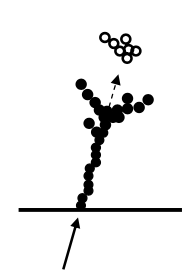
\includegraphics[width=0.2\textwidth]{LCDetectorsAndPFlow/Plots/Pictures/Association6.png}}
\hspace{5mm}
\subfloat[]{\label{fig:association7}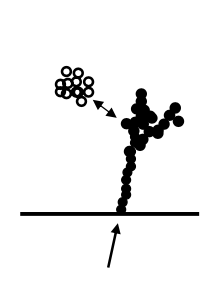
\includegraphics[width=0.2\textwidth]{LCDetectorsAndPFlow/Plots/Pictures/Association7.png}}
\hspace{5mm}
\subfloat[]{\label{fig:association8}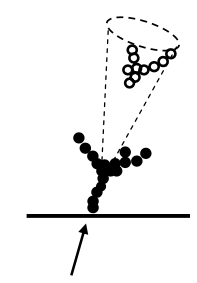
\includegraphics[width=0.2\textwidth]{LCDetectorsAndPFlow/Plots/Pictures/Association8.png}}
\hspace{5mm}
\subfloat[]{\label{fig:association9}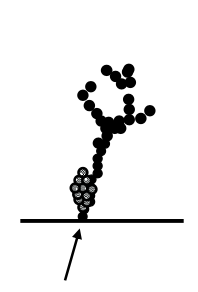
\includegraphics[width=0.2\textwidth]{LCDetectorsAndPFlow/Plots/Pictures/Association9.png}}
\caption[The main topological rules for cluster merging: \protect\subref{fig:association1} looping track segments; \protect\subref{fig:association2} track segments with gaps; \protect\subref{fig:association3} track segments pointing to hadronic showers; \protect\subref{fig:association4} track-like neutral clusters pointing back to a hadronic shower; \protect\subref{fig:association5} back-scattered tracks from hadronic showers; \protect\subref{fig:association6} neutral clusters which are close to a charged cluster; \protect\subref{fig:association7} a neutral cluster near a charged cluster; \protect\subref{fig:association8} cone association; and \protect\subref{fig:association9} recovery of photons which overlap with a track segment.  In each case the arrow indicates the track, the filled points represent the hits in the associated cluster and the open points represent hits in the neutral cluster.  \textcolor{blue}{Charged clusters are defined by having an associated charged particle track, while neutral clusters have no associated tracks.} Figures taken from \cite{arXiv:0907.3577}.]{The main topological rules for cluster merging: \protect\subref{fig:association1} looping track segments; \protect\subref{fig:association2} track segments with gaps; \protect\subref{fig:association3} track segments pointing to hadronic showers; \protect\subref{fig:association4} track-like neutral clusters pointing back to a hadronic shower; \protect\subref{fig:association5} back-scattered tracks from hadronic showers; \protect\subref{fig:association6} neutral clusters which are close to a charged cluster; \protect\subref{fig:association7} a neutral cluster near a charged cluster; \protect\subref{fig:association8} cone association; and \protect\subref{fig:association9} recovery of photons which overlap with a track segment.  In each case the arrow indicates the track, the filled points represent the hits in the associated cluster and the open points represent hits in the neutral cluster.  \textcolor{blue}{Charged clusters are defined by having an associated charged particle track, while neutral clusters have no associated tracks.}. Figures taken from \cite{arXiv:0907.3577}.}
\label{fig:associations}
\end{figure} 

The application of the pattern recognition algorithms in PandoraPFA when combined with a highly segmented detector make particle flow calorimetry a reality.  In turn this provides excellent jet energy resolution for studying many interesting physics processes at the linear collider experiments.

%======================================================================================== 
%======================================================================================== 

\section{Performance}
\label{sec:performance}
The fundamental principle of particle flow calorimetry is to measure the energy of a particle passing through a detector in whichever sub-detector offers the best energy resolution.  For particle collider experiments, this involves measuring the momenta of charged particles using the curvature of the track they create in the detector.  This offers extremely good energy resolution in comparison to the traditional calorimetric approach.  

As many physics processes of interest at the linear collider involve multi-jet final states \cite{Abramowicz:2016zbo}, good jet energy resolution is a crucial aspect of detector performance.    As shown in chapter \ref{chap:PhysicsAnalysis}, the sensitivity of the linear collider experiments to areas of new physics can be determined using reconstructed jet energies.  Furthermore, parameters derived from the energy measurements of jets are extremely useful for identification of physics channels of interest.  Therefore, a key metric for describing detector performance is the jet energy resolution.  Jet energy resolution in particular can benefit from the application of particle flow calorimetry because $\approx 70 \%$ of the energy of jets is carried in the form of charged particles.  As particle flow calorimetry aims to measure the energy of charged particles using the tracker, it has the potential to offer extremely large benefits when measuring jet energies in comparison to the traditional calorimetric approach.  

%========================================================================================

\subsection{Jet Energy Resolution}
The jet energy resolution in these studies was determined through the simulation of off-mass shell Z boson events decaying to light quarks (u, d, s).  PYTHIA version 6.4 \cite{Sjostrand:2006za}, which had been trained on fragmentation data from the OPAL experiment \cite{Alexander:1995bk}, was used to generate these events.  The decay of tau leptons appearing in the events was simulated using TAUOLA \cite{Was:2000st}.  Detector simulation and event reconstruction was carried out as described in sections \ref{sec:simulation} and \ref{sec:reconstruction} respectively.  

As the Z boson in these events is produced at rest, the typical decays form two mono-energetic jets that are produced back-to-back as shown in figure \ref{fig:500GeVzudsevtdisplay}.  Only events where $|\text{cos}(\theta)| < 0.7$, where $\theta$ is the polar angle of the quarks, are used in the jet energy resolution calculation.  This ensures that little energy is lost down the beam axis.  Using these events, the jet energy resolution was calculated as follows: 
\begin{equation} 
\frac{\text{RMS}_{90}(E_{j})}{\text{Mean}_{90}(E_{j})} = \frac{\text{RMS}_{90}(E_{jj})}{\text{Mean}_{90}(E_{jj})} \times \sqrt{2} \text{ ,}
\end{equation}
\noindent where $E_{jj}$ is the total reconstructed energy.  The variables $\text{Mean}_{90}(E_{jj})$ and $\text{RMS}_{90}(E_{jj})$ are the mean and root mean squared (RMS) of the $E_{jj}$ distribution respectively.  They are calculated across the range of $E_{jj}$ with the smallest RMS containing at least 90\% of the data.  This definition is used to remove the effect of outliers in the distribution \cite{arXiv:0907.3577}.  If all associations between charged particle tracks and calorimeter clusters were correctly made, the reconstructed jet energy distribution would be Gaussian.  However, the effect of confusion on certain events will distort this distribution and broaden the tails significantly.  If the full range were to be used in the jet energy resolution calculation, the effect of these tails is overinflated.  When the distribution of reconstructed jet energies is truncated to the narrowest range that contains at least $90\%$ of the data, the effect of these tails can be negated.  This removes events where confusion is dominant, which makes the jet energy resolution metric far more robust and representative of the bulk of the data.  

\begin{figure}[h!]
\centering
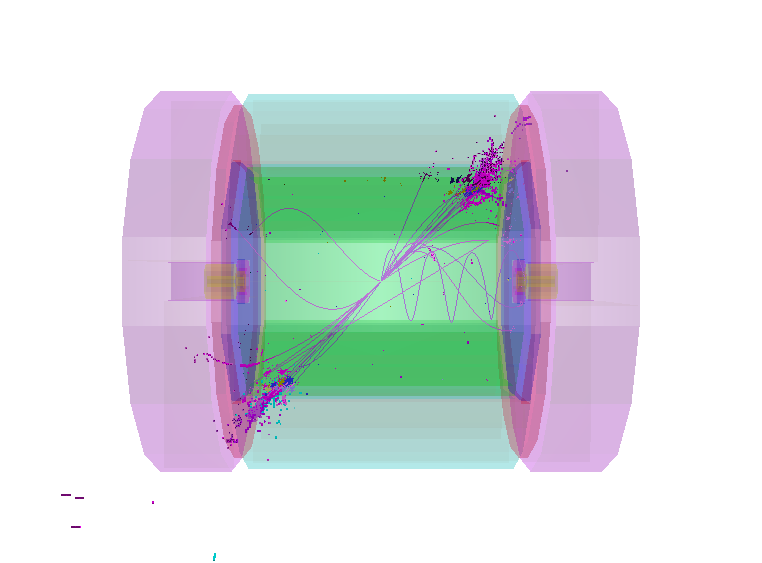
\includegraphics[width=0.75\textwidth]{OptimisationStudies/Plots/MethodDescription/500GeVEvent.png}
\caption[\textcolor{blue}{A} 500~GeV di-jet Z$\rightarrow$uds event display for \textcolor{blue}{the} nominal ILD detector.]{\textcolor{blue}{A} 500~GeV di-jet Z$\rightarrow$uds event display for \textcolor{blue}{the} nominal ILD detector.}
\label{fig:500GeVzudsevtdisplay}
\end{figure} 

\begin{figure}[h!]
\centering
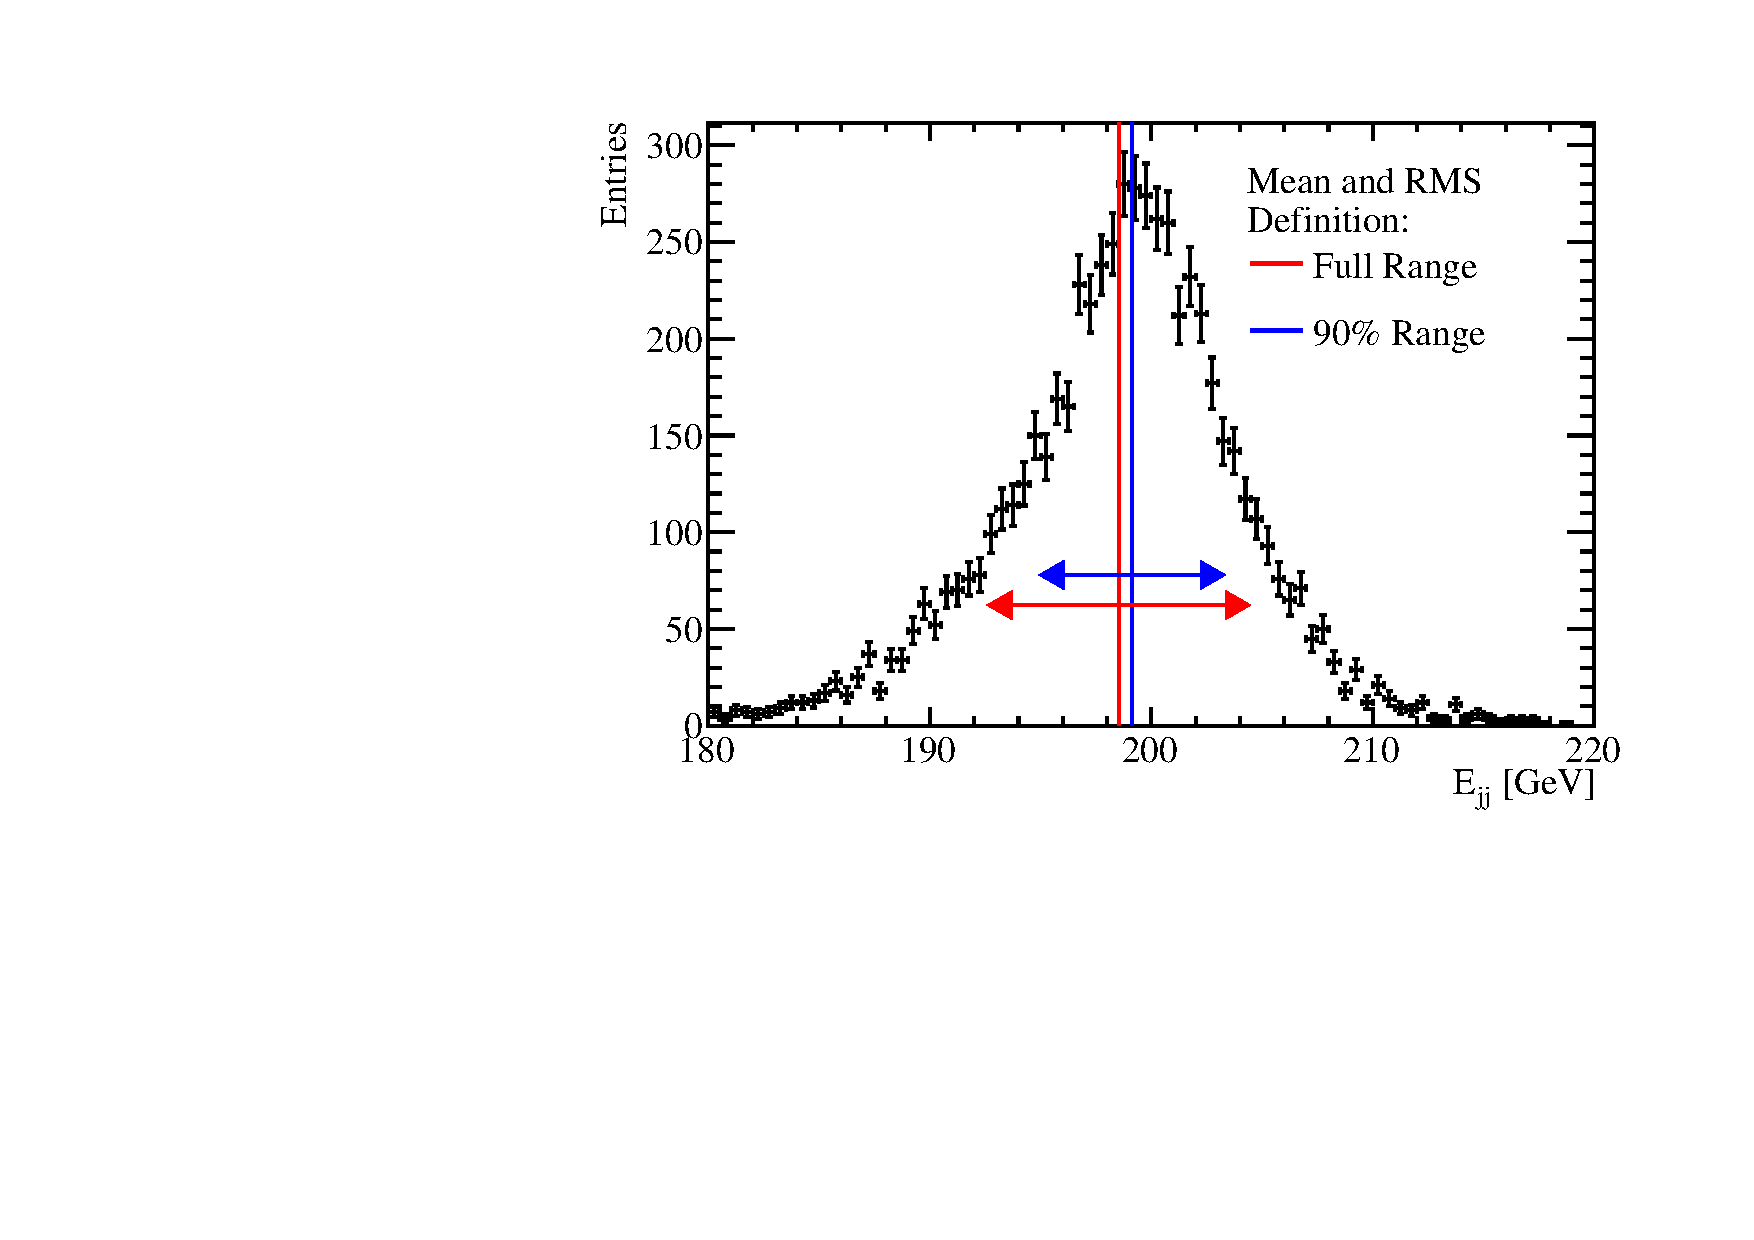
\includegraphics[width=0.5\textwidth]{OptimisationStudies/Plots/MethodDescription/RMS90Plot.pdf}
\caption[Definition of jet energy resolution.   Reconstructed jet energy for 200~GeV di-jet Z$\rightarrow$uds events for nominal ILD detector.  The solid vertical line shows the mean of the distribution and the horizontal arrows indicate the mean $\pm$ the root mean square (RMS) of the distribution.  The red and blue lines represent the mean and RMS calculated using the full range and 90\% of the full range with the smallest RMS.]{Definition of jet energy resolution.   Reconstructed jet energy for 200~GeV di-jet Z$\rightarrow$uds events for nominal ILD detector.  The solid vertical line shows the mean of the distribution and the horizontal arrows indicate the mean $\pm$ the root mean square (RMS) of the distribution.  The red and blue lines show the mean and RMS calculated using the full range and 90\% of the full range with the smallest RMS respectively.}
\label{fig:rms90defintion}
\end{figure} 

An example of the application of this metric can be found in figure \ref{fig:rms90defintion}.  In this example $\text{RMS}(E_{jj})$, the RMS calculated using the full range, is 5.8~GeV, while $\text{RMS}_{90}(E_{jj})$, the RMS using the reduced range, is 4.1~GeV.  This corresponds to a reduction in the jet energy resolution from $4.1\%$ to $2.9\%$, which clearly shows an overemphasis of the tails of the distribution when using the full jet energy range.

In the subsequent analysis a range of di-jet energies were considered ranging from the Z mass, 91~GeV, to the nominal running energy of the ILC, 500~GeV.  Each event sample contained 10,000 events generated isotropically so that, given the polar angle cut, approximately 7,000 events contribute to the jet energy resolution calculation. 

%========================================================================================

\subsection{Decomposition of the Jet Energy Resolution}
\label{sec:jerdecomposition}
It is possible to gain additional insight into the detector performance by cheating the pattern recognition.  Cheating the pattern recognition involves using Monte-Carlo (MC) information to correctly cluster calorimeter hits together and associate them to charged particle tracks.  This has the effect of removing confusion from the reconstruction.  By comparing the detector performance obtained from the standard and cheated reconstructions, it is possible to decompose the detector performance into two terms; one related exclusively to the intrinsic energy resolution of the detector and another related to the pattern recognition confusion.  The additional information this provides is extremely useful for characterising changes to the overall detector performance.  

The intrinsic energy resolution contribution to the jet energy resolution is determined by fully cheating the pattern recognition; in this case all confusion is negated.  The total confusion is defined as the quadrature difference between the jet energy resolution using the standard reconstruction and this fully cheated reconstruction.  Furthermore, it is possible to cheat the pattern recognition associated with individual types of particles.  This is particularly useful for studies related to the ECal as, by cheating the photon pattern recognition, it is possible to isolate the confusion associated with photons.  The photon confusion is defined as the quadrature difference between the jet energy resolution using the standard reconstruction and the reconstruction where the photon pattern recognition is cheated.  Examples of the calculation of the various confusion terms defined above are given in table \ref{table:confusioncalculation}.

\begin{table}[h!]
\centering
\begin{tabular}{ l r}
\hline
Reconstruction & Jet Energy Resolution [\%] \\
\hline
Standard Reconstruction (No MC Information) & $a = 2.97\pm0.05$ \\
Cheating Entire Reconstruction & $b = 1.69\pm0.02$ \\
Confusion & $\sqrt{a^{2}-b^{2}} = 2.45\pm0.05$ \\
\hline
Cheating Photon Reconstruction & $c = 2.73\pm0.04$ \\
Photon Confusion & $\sqrt{a^{2}-c^{2}} =1.18\pm0.06$ \\
\hline
\end{tabular}
\caption[Example calculation of the confusion contributions to the jet energy resolution.  These jet energy resolutions are for 250~GeV jets using the nominal ILD detector model and are calculated using the range of jet energies with the smallest RMS containing at least 90\% of the data.]{Example calculation of the confusion contributions to the jet energy resolution.  These jet energy resolutions are for 250~GeV jets using the nominal ILD detector model and are calculated using the range of jet energies with the smallest RMS containing at least 90\% of the data.}
\label{table:confusioncalculation}
\end{table}

A common feature that is observed in these calibration studies is that as the intrinsic energy resolution of a calorimeter improves, the effect of confusion is reduced.  This occurs as a better energy resolution means more precise comparisons can be made between the energy of a cluster of calorimeter hits and the momentum of any charged particle tracks associated to it.  Comparisons such as these are made by PandoraPFA to determine whether the track cluster associations that have been made are consistent.  If a large discrepancy is observed between the cluster energy and track momenta, the clustering of calorimeter hits is modified until a consistent association can be made.  For more details on this comparison see chapter \ref{chap:pflowandlcdetectors}.  This consistency check vastly reduces the number of errors made when clustering calorimeter hits and associating charged particle tracks to those clusters i.e. the confusion.  Therefore, improving the precision of this consistency check, by improving the energy resolution, reduces the effect of confusion.  

%========================================================================================

\subsection{Single Particle Energy Resolution}
The energy resolution for individual particles is crucial for a number of physics studies of interest to the linear collider, such as photon energy resolutions in the study of anomalous triple and quartic gauge couplings \cite{Chatrchyan:2013fya,ATLAS:2012mec,Chatrchyan:2014bza}.  Therefore, photon and $K^{0}_{L}$ energy resolutions, alongside the jet energy resolution, will be considered in these optimisation studies.  As both photon and $K^{0}_{L}$ are uncharged, their energy measurements will be made using the calorimeters as opposed to the tracker.  Photons are a natural choice of particle to consider as they are particularly relevant for several physics studies and, as they are largely contained within the ECal, they will be highly sensitive to changes in the ECal performance.  $K^{0}_{L}$s were used as, analogously to photons and the ECal, their energies are primarily measured using the HCal.  In general, neutral hadron energy resolutions are less crucial to physics studies, however, they do make crucial contribution to the jet energy resolution that should not be overlooked.  The reported photon energy resolutions were determined using events containing a single 100~GeV photon, while the $K^{0}_{L}$ energy resolutions were determined using events containing a single 50~GeV $K^{0}_{L}$.  These energies were chosen to be as large as possible, to maximise sampling of the calorimeter response, while minimising the effect of energy leakage from the ECal to the HCal for the photons and leakage of energy out of the rear of the HCal for the $K^{0}_{L}$ events.

The energy resolution for these single particle samples is determined using a Gaussian fit to the reconstructed energy distributions.  To aid convergence, the fit was applied to the narrowest range of the reconstructed energy distribution containing at least 75\% of the data.  The single particle energy resolution is defined as the standard deviation divided by the mean of the fitted Gaussian.  For each energy resolution calculation, a total of 10,000 events were used to populate the reconstructed energy distribution.  For clarity, a cut of $|\text{cos}(\theta)| < 0.7$ was applied to veto events where particles travelled down the beam pipe or where they passed through the barrel/endcap overlap region.  An example of the reconstructed energy distributions for 100~GeV photons and 50~GeV $K^{0}_{L}$s, alongside the Gaussian fits used to determine the energy resolutions, are shown in figure \ref{fig:singleparticleenergyhists}.  The errors quoted on single particle energy resolutions are determined by propagating the errors reported from the Gaussian fit into the resolution calculation.  

\begin{figure}[h!]
\centering
\subfloat[]{\label{fig:kaonsingleparticleenergyhist}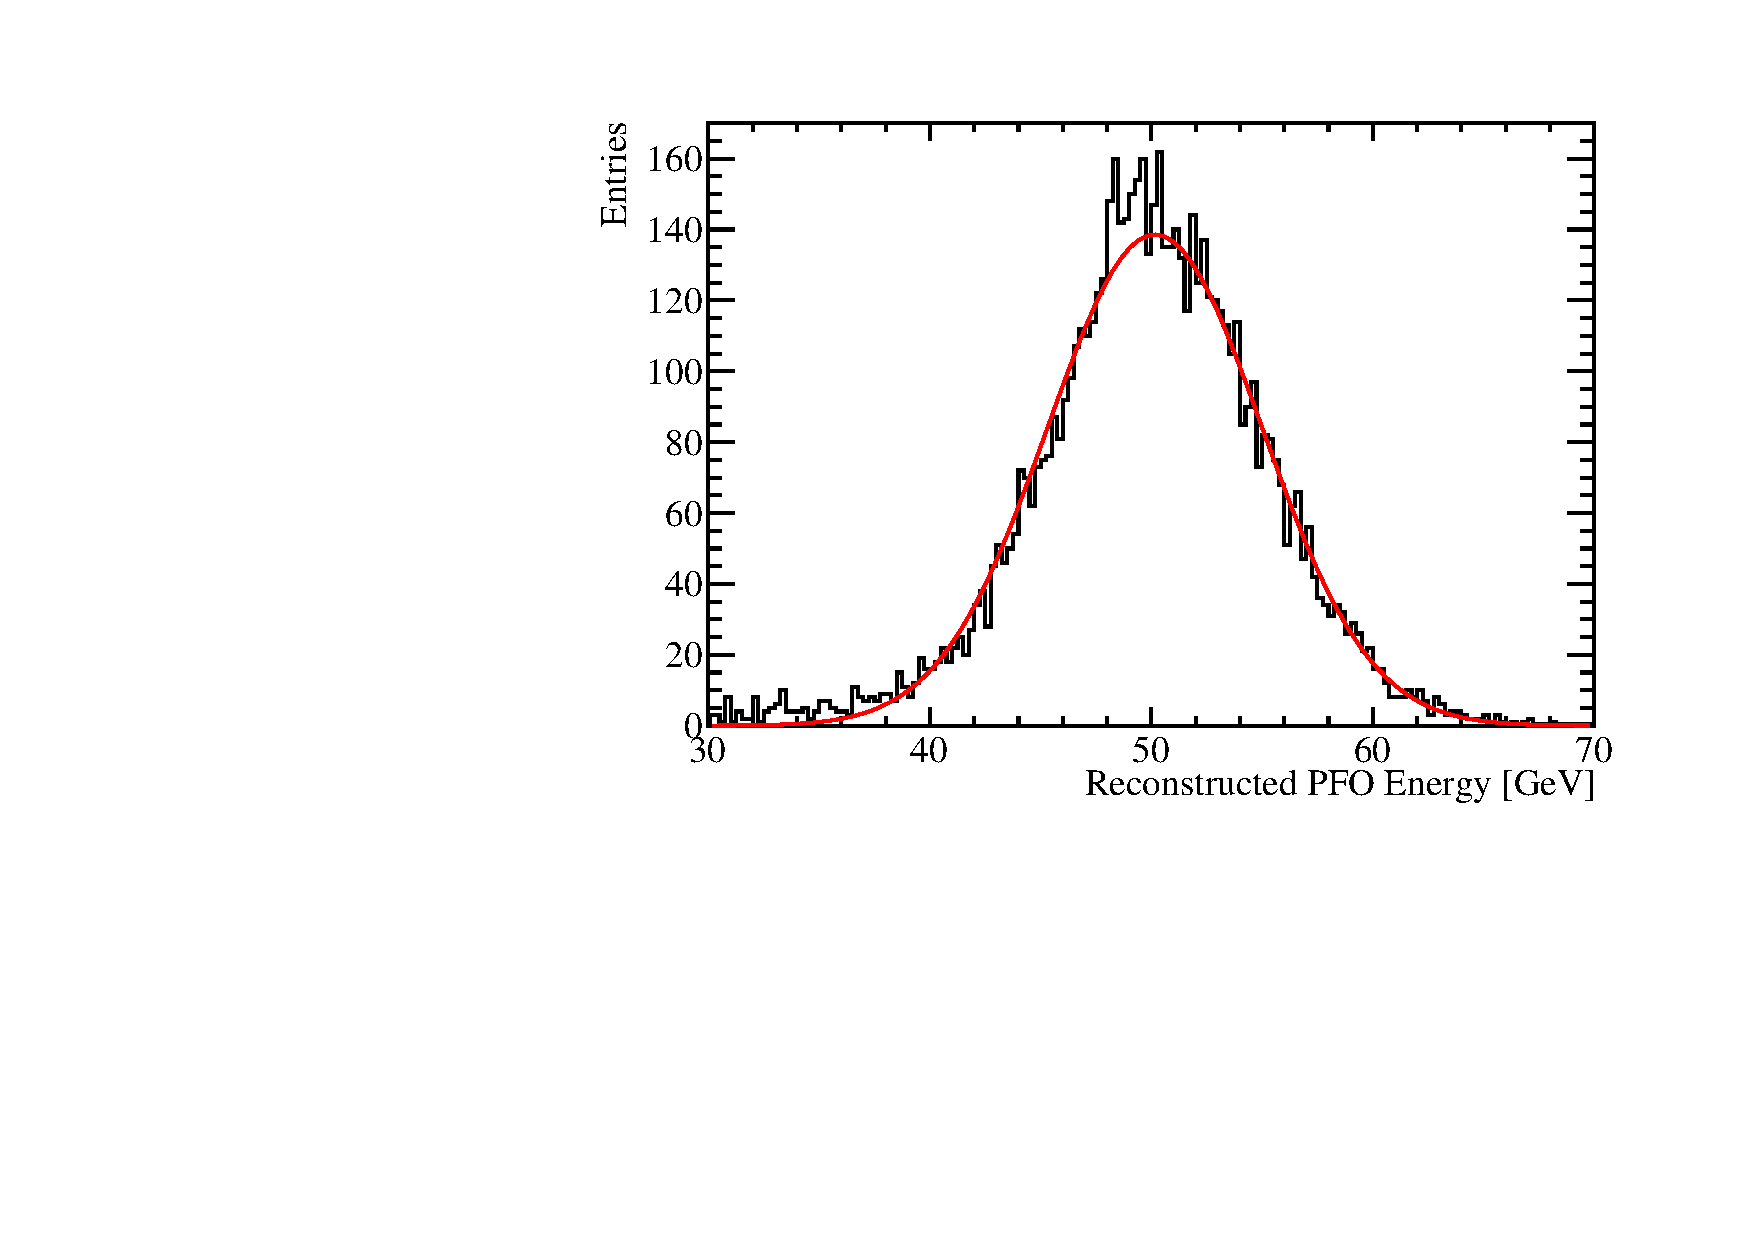
\includegraphics[width=0.5\textwidth]{OptimisationStudies/Plots/EnergyResolution/EKaon0L_50GeV.pdf}}
\subfloat[]{\label{fig:photonsingleparticleenergyhist}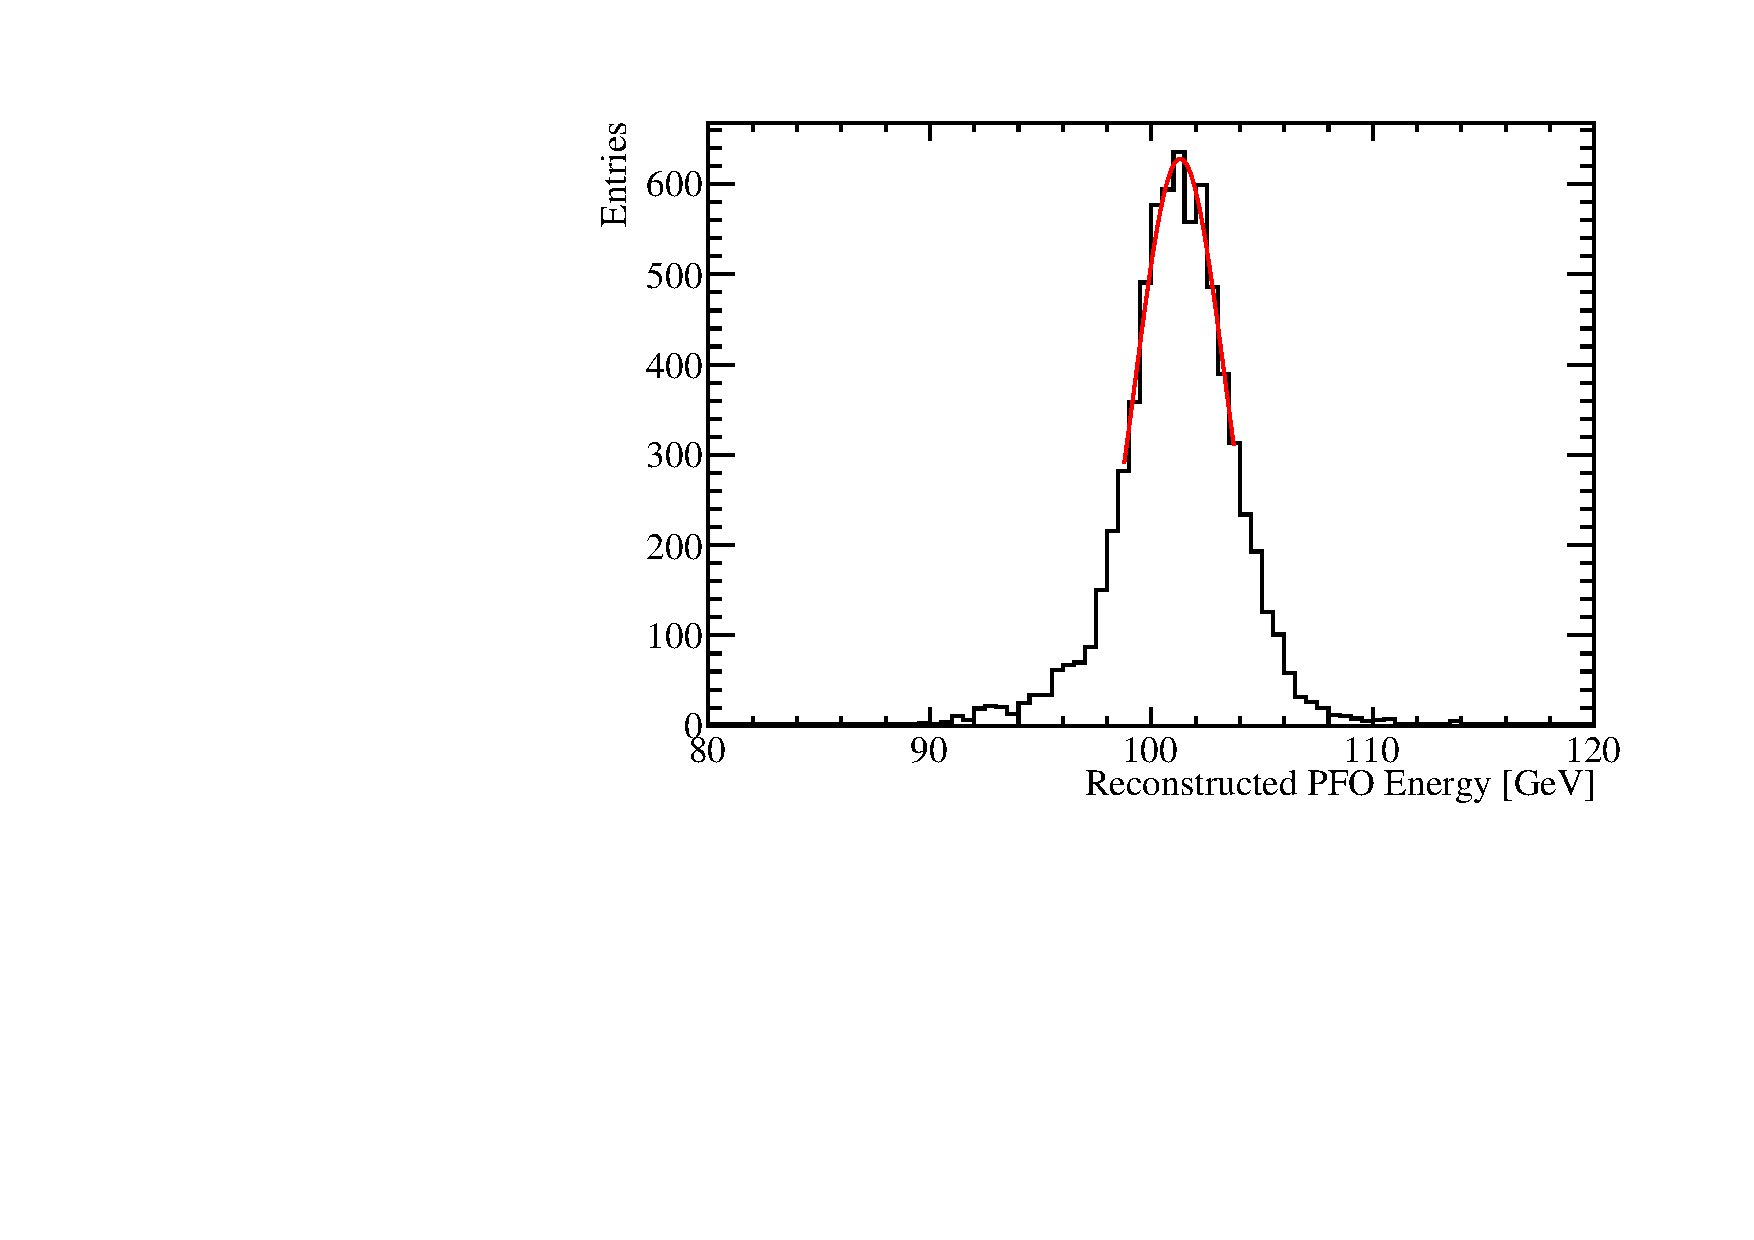
\includegraphics[width=0.5\textwidth]{OptimisationStudies/Plots/EnergyResolution/EPhoton_100GeV.pdf}}
\caption[The reconstructed energy distribution for \protect\subref{fig:kaonsingleparticleenergyhist} 50~GeV $K^{0}_{L}$ and \protect\subref{fig:photonsingleparticleenergyhist} 100~GeV photons.  The red line shows a Gaussian fit used to parameterise the detector performance.  The fit was applied to the truncated range of the reconstructed PFO energy distribution containing at least 75\% of the data with the narrowest RMS.  The nominal ILD model was used in this simulation.]{The reconstructed energy distribution for \protect\subref{fig:kaonsingleparticleenergyhist} 50~GeV $K^{0}_{L}$ and \protect\subref{fig:photonsingleparticleenergyhist} 100~GeV photons.  The red line shows a Gaussian fit used to parameterise the detector performance.  The fit was applied to the truncated range of the reconstructed PFO energy distribution containing at least 75\% of the data with the narrowest RMS.  The nominal ILD model was used in this simulation.}
\label{fig:singleparticleenergyhists}
\end{figure}

%========================================================================================
%========================================================================================

\section{Summary of ILD Detector Performance}
\label{sec:nominaldetectorperformance}
The following section outlines the nominal ILD detector performance using the metrics outlined in section \ref{sec:performance}.  

The reconstructed energy distributions for particles whose energies are measured using calorimeters will be Gaussian.  This is the case for sampling calorimeters as the active material in each calorimeter hit essentially counts the number of charged particle tracks passing through it, or possible the number of photons for scintillator options.  An estimation of the total energy deposited in a calorimeter hit, including the absorber material, can be made based upon this number of tracks or photons.  For more details on how this estimation is made see chapter \ref{chap:energyestimators}.  Finally, the energy of the entire particle shower is estimated by grouping together calorimeter hits and summing their energy.  As each calorimeter hit's energy is an independent random measurement the particle shower energy will, by the central limit theorem, have a Gaussian distribution.  

The energy of a calorimeter hit is obtained by counting the number of charged particle tracks or photons found in the active material of the calorimeter, therefore, Poisson statistics govern the distribution of calorimeter hit energies.  If the mean of the distribution of the energy of a cluster of calorimeter hits is $\lambda = N$, where $N$ is the mean number of objects that are measured in the calorimeters, the standard deviation of that distribution is $\sigma = \sqrt{\lambda} = \sqrt{N}$ and the energy resolution is $\sigma / \lambda = 1 / \sqrt{N}$.  As the total shower energy, $E_{Reco}$, is proportional to $N$, the energy resolution for a particle shower in an ideal calorimeter is $\sigma_{Reco} / E_{Reco} = a / \sqrt{E_{Reco}}$.  In reality, it is typical to express the energy resolution of a calorimeter in the following form
%
\begin{equation} 
\frac{\sigma_{Reco}}{E_{Reco}} = \frac{a}{\sqrt{E_{Reco}}} \oplus b \oplus \frac{c}{E_{Reco}}\text{ ,}
\end{equation}
%
\noindent where the $b$ term is a constant term that accounts for a variety of instrumental effects that do not depend on energy, e.g. mechanical imperfections, and the $c$ term accounts for electrical noise \cite{Fabjan:2003aq}.  Here, $\oplus$ denotes the quadrature sum of variables.  

Prototypes of the various ILD calorimeter options have been constructed and validated using test beam measurements.  The energy resolution of the ILD ECal, determined from test beam measurements, was parameterised as $16.6\% / \sqrt{E_{Reco}(\text{GeV})} \oplus 1.1 \%$ for the silicon option and $12.9 \% / \sqrt{E_{Reco}(\text{GeV})} \oplus 1.2 \%$ for the scintillator option \cite{Behnke:2013lya}.  The electrical noise was deemed sufficiently small that the $c$ term in the parameterisation could be neglected in both cases.  These results were determined using an $\text{e}^{-}$ test beam with energies ranging up to $\approx 40$~GeV.  This parametrisation is compared to the full ILD detector simulation in figures \ref{fig:ecalsinominalres} and \ref{fig:ecalscnominalres} for the silicon and scintillator ECal options respectively.  The test beam parameterisation of the energy resolution for the silicon ECal option is almost identical to the energy resolution observed in the full simulation.  At very high energies, $\approx 500$~GeV, the ECal is no longer sufficient to fully contain the photons and so leakage of energy into the HCal leads to a minor degradation in the simulated energy resolution.  This accounts for the worse energy resolution seen in the full simulation when compared to an extrapolation of the test beam parameterisation at high energies.  The test beam parameterisation of the energy resolution for the scintillator ECal option is significantly better than that observed in the full simulation, which is most likely due to an imperfect implementation of the scintillator ECal within the full detector simulation.  The photon energy resolutions seen in the full ILD simulation are similar for the silicon and scintillator ECal options.      

Similarly, the energy resolution, determined from test beam measurements, for the nominal ILD HCal was parameterised as $57.6 \% / \sqrt{E_{Reco}(\text{GeV})} \oplus 1.6 \%$ \cite{Adloff:2012gv}.  A comparison between this test beam parameterisation and the full ILD simulation, using the silicon ECal option, is shown in figure \ref{fig:hcalnominalres}.  The test beam measurements were made using $\pi^{\pm}$s with energies ranging from 10 to 80~GeV, while the full ILD simulation used $K^{0}_{L}$s ranging from 10 to 100~GeV.  The deviation between the test beam parameterisation and the full ILD simulation, which grows as the $K^{0}_{L}$ energy increases, is most likely due to the treatment of energy deposits leaking out of the back of the HCal.  In the test beam studies, to minimise the effect of leakage, events were only considered if the particle showers started developing at the front of the HCal.  In the full simulation studies, all particle showers were used, which means some energy will have leaked out of the back of the calorimeters and been deposited in the uninstrumented solenoid region of the detector, resulting in a degradation in the energy resolution.   

Figure \ref{fig:jernominalres} shows the jet energy resolution as a function of jet energy for the full ILD simulation.  Alongside this, the intrinsic energy resolution and confusion contributions to the jet energy resolution are also presented.  The jet energy resolution at low energies is dominated by the intrinsic energy resolution of the detector, while at high energies it is dominated by the effect of confusion.  This is to be expected because the intrinsic energy resolution of the calorimeters is approximately proportional to $1 / \sqrt{E_{Reco}}$.  On the other hand, confusion grows with energy because increasing energy leads to more dense event topologies, which makes pattern recognition more challenging.  The total jet energy resolution for the ILD detector are sufficiently small, $\sigma_{E_{j}} / E_{j} \lesssim 3.8\%$ \cite{Behnke:2013lya, arXiv:0907.3577, Linssen:2012hp}, across the energy range considered to make separation of the hadronic decays of the W and Z bosons possible, which is one of the key requirements for the future linear collider.

\begin{figure}[h!]
\centering
\subfloat[]{\label{fig:ecalsinominalres}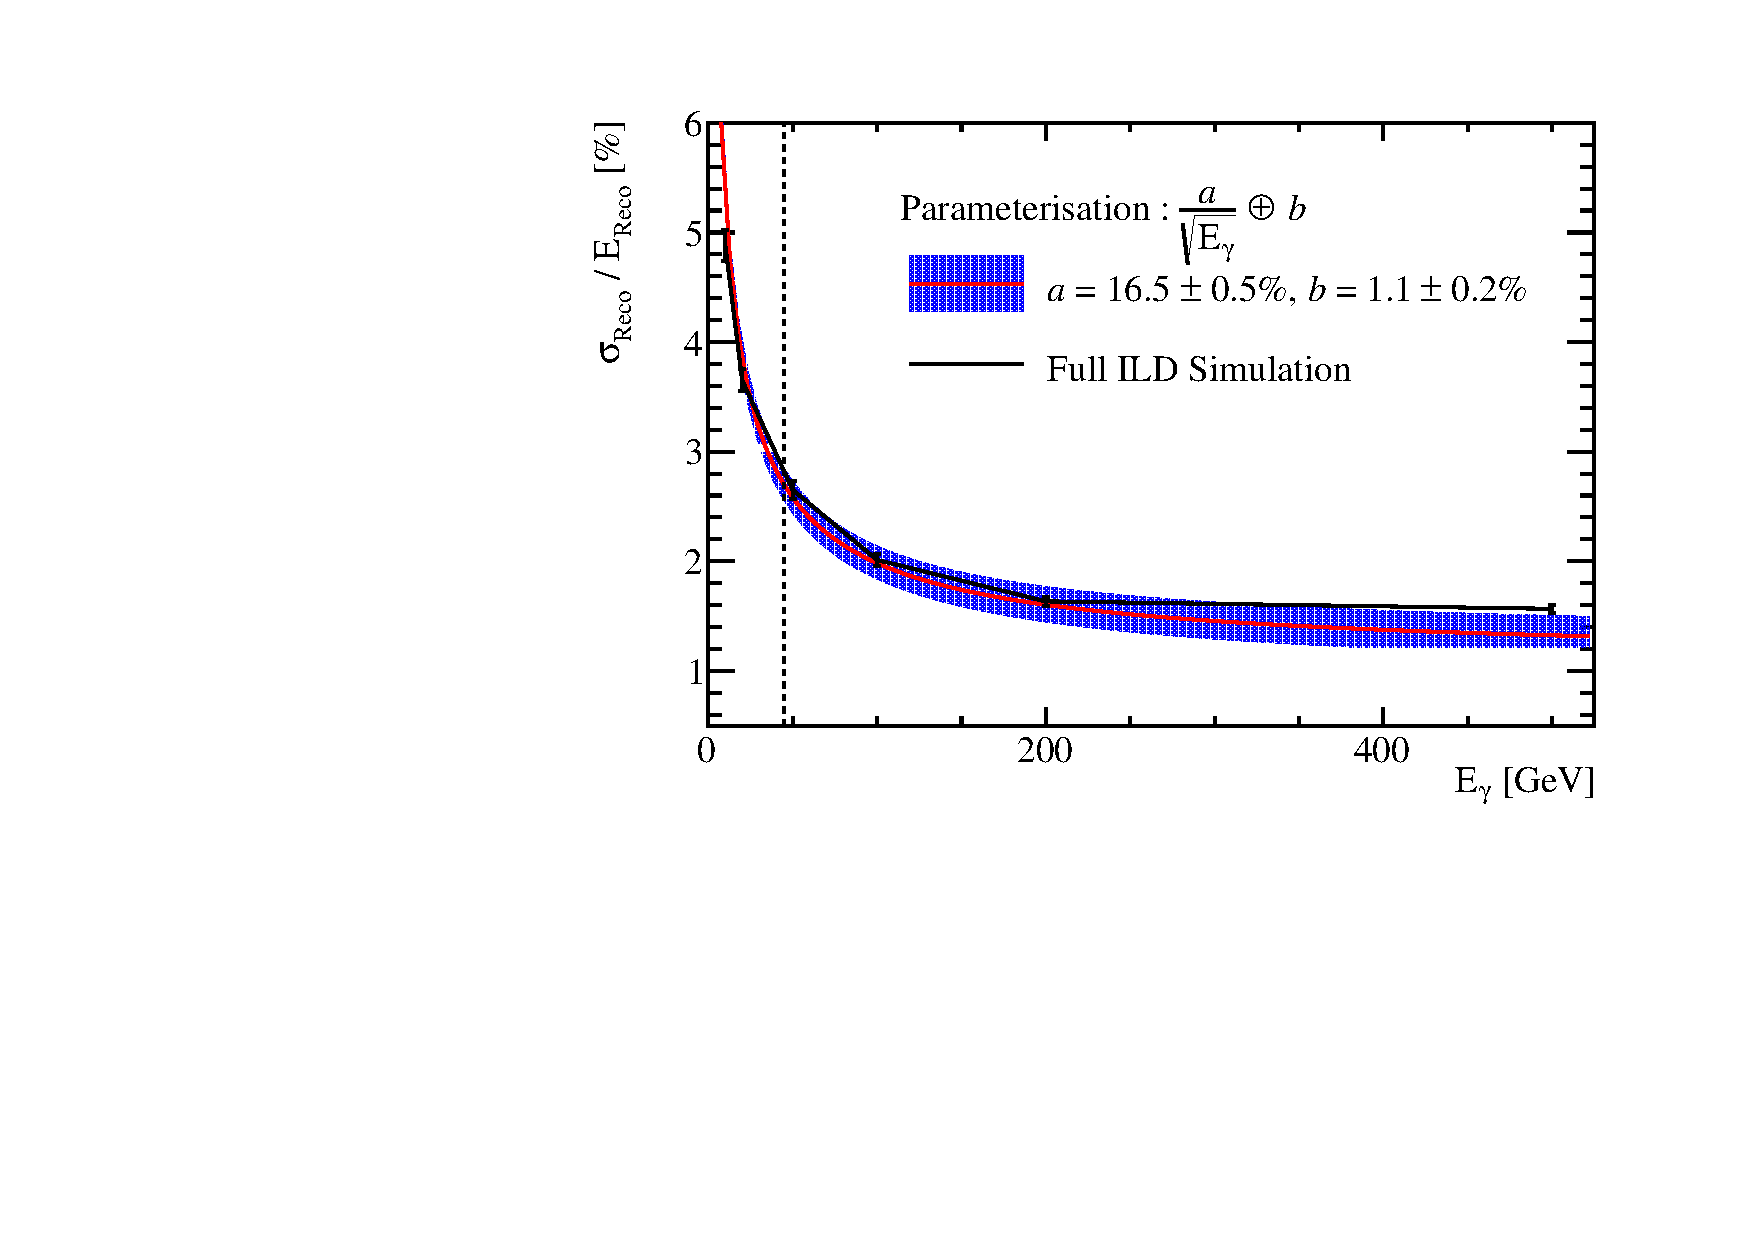
\includegraphics[width=0.5\textwidth]{OptimisationStudies/Plots/EnergyResolution/ER_vs_EGamma_SiECal.pdf}}
\subfloat[]{\label{fig:ecalscnominalres}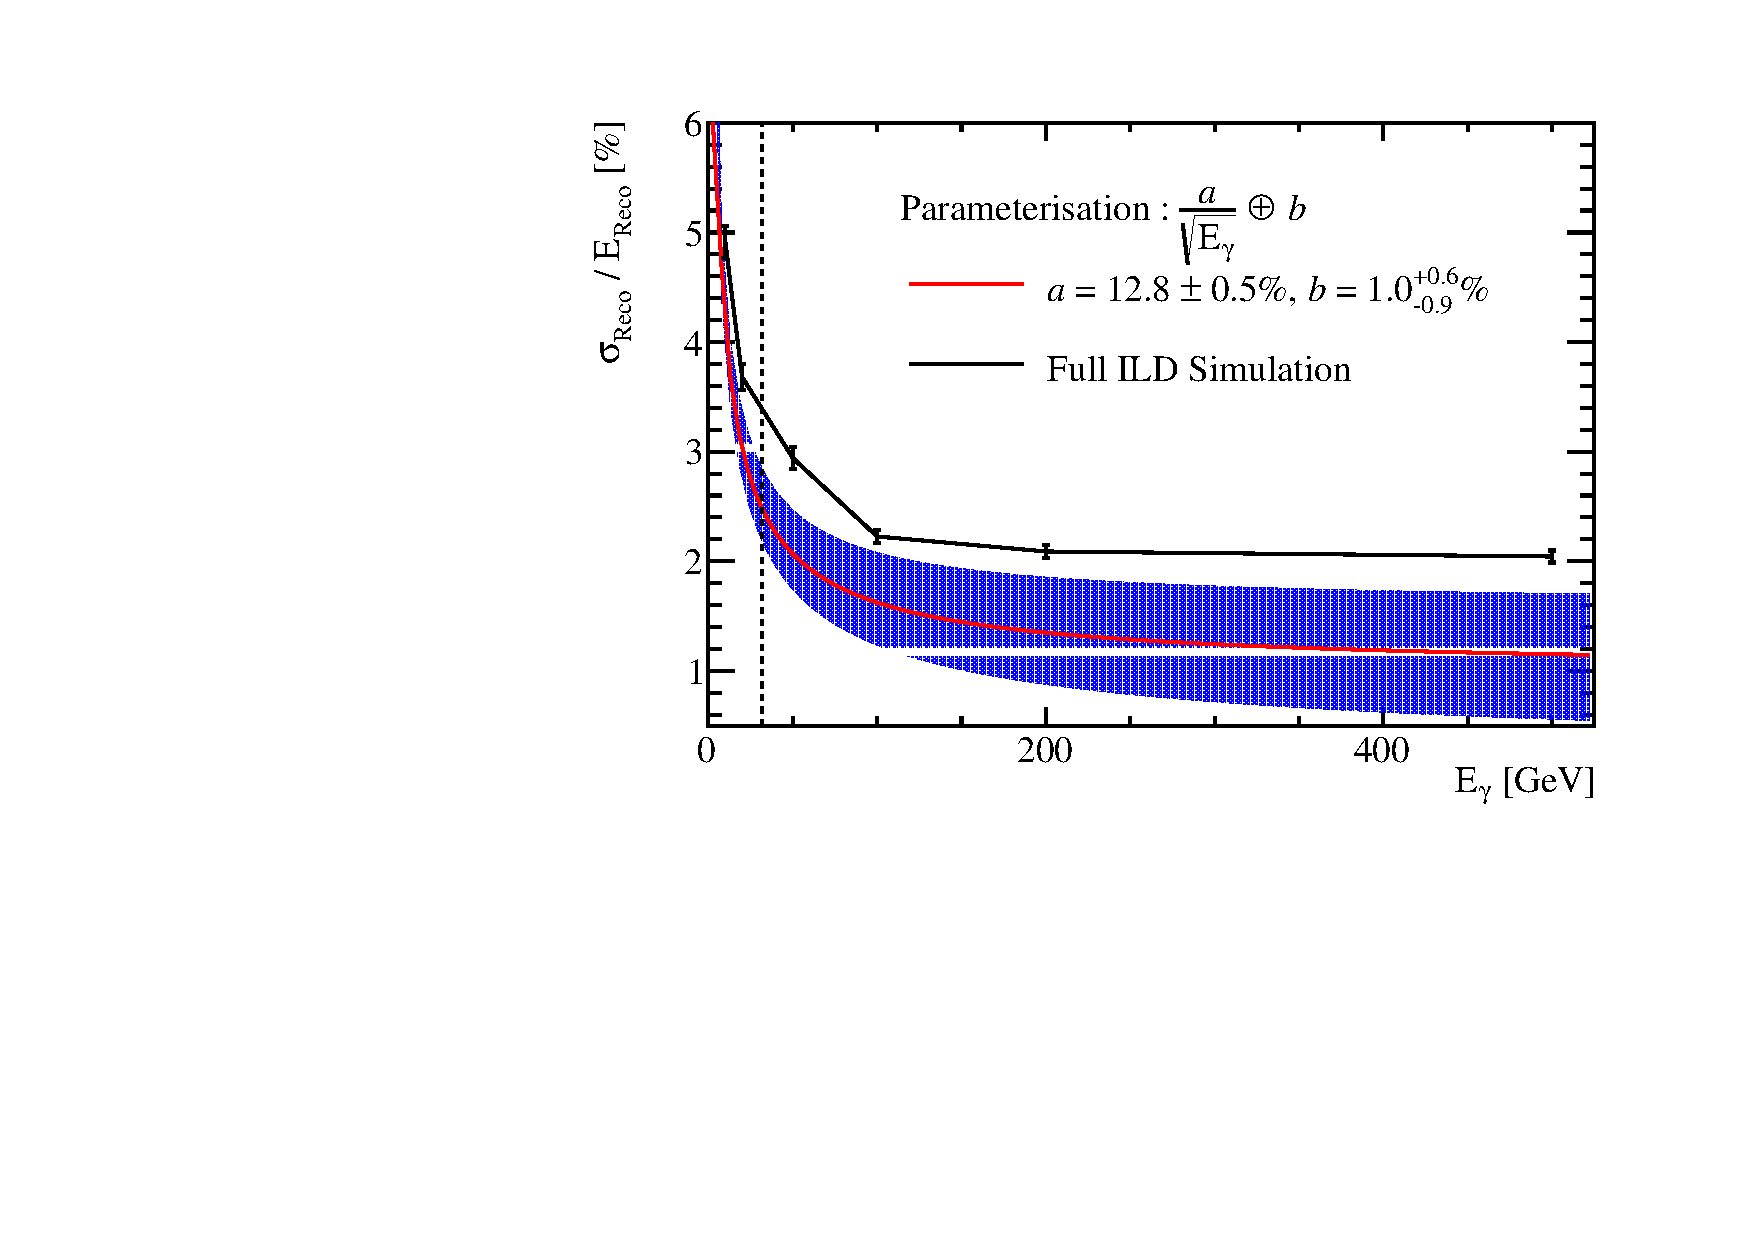
\includegraphics[width=0.5\textwidth]{OptimisationStudies/Plots/EnergyResolution/ER_vs_EGamma_ScECal.pdf}}\\
\subfloat[]{\label{fig:hcalnominalres}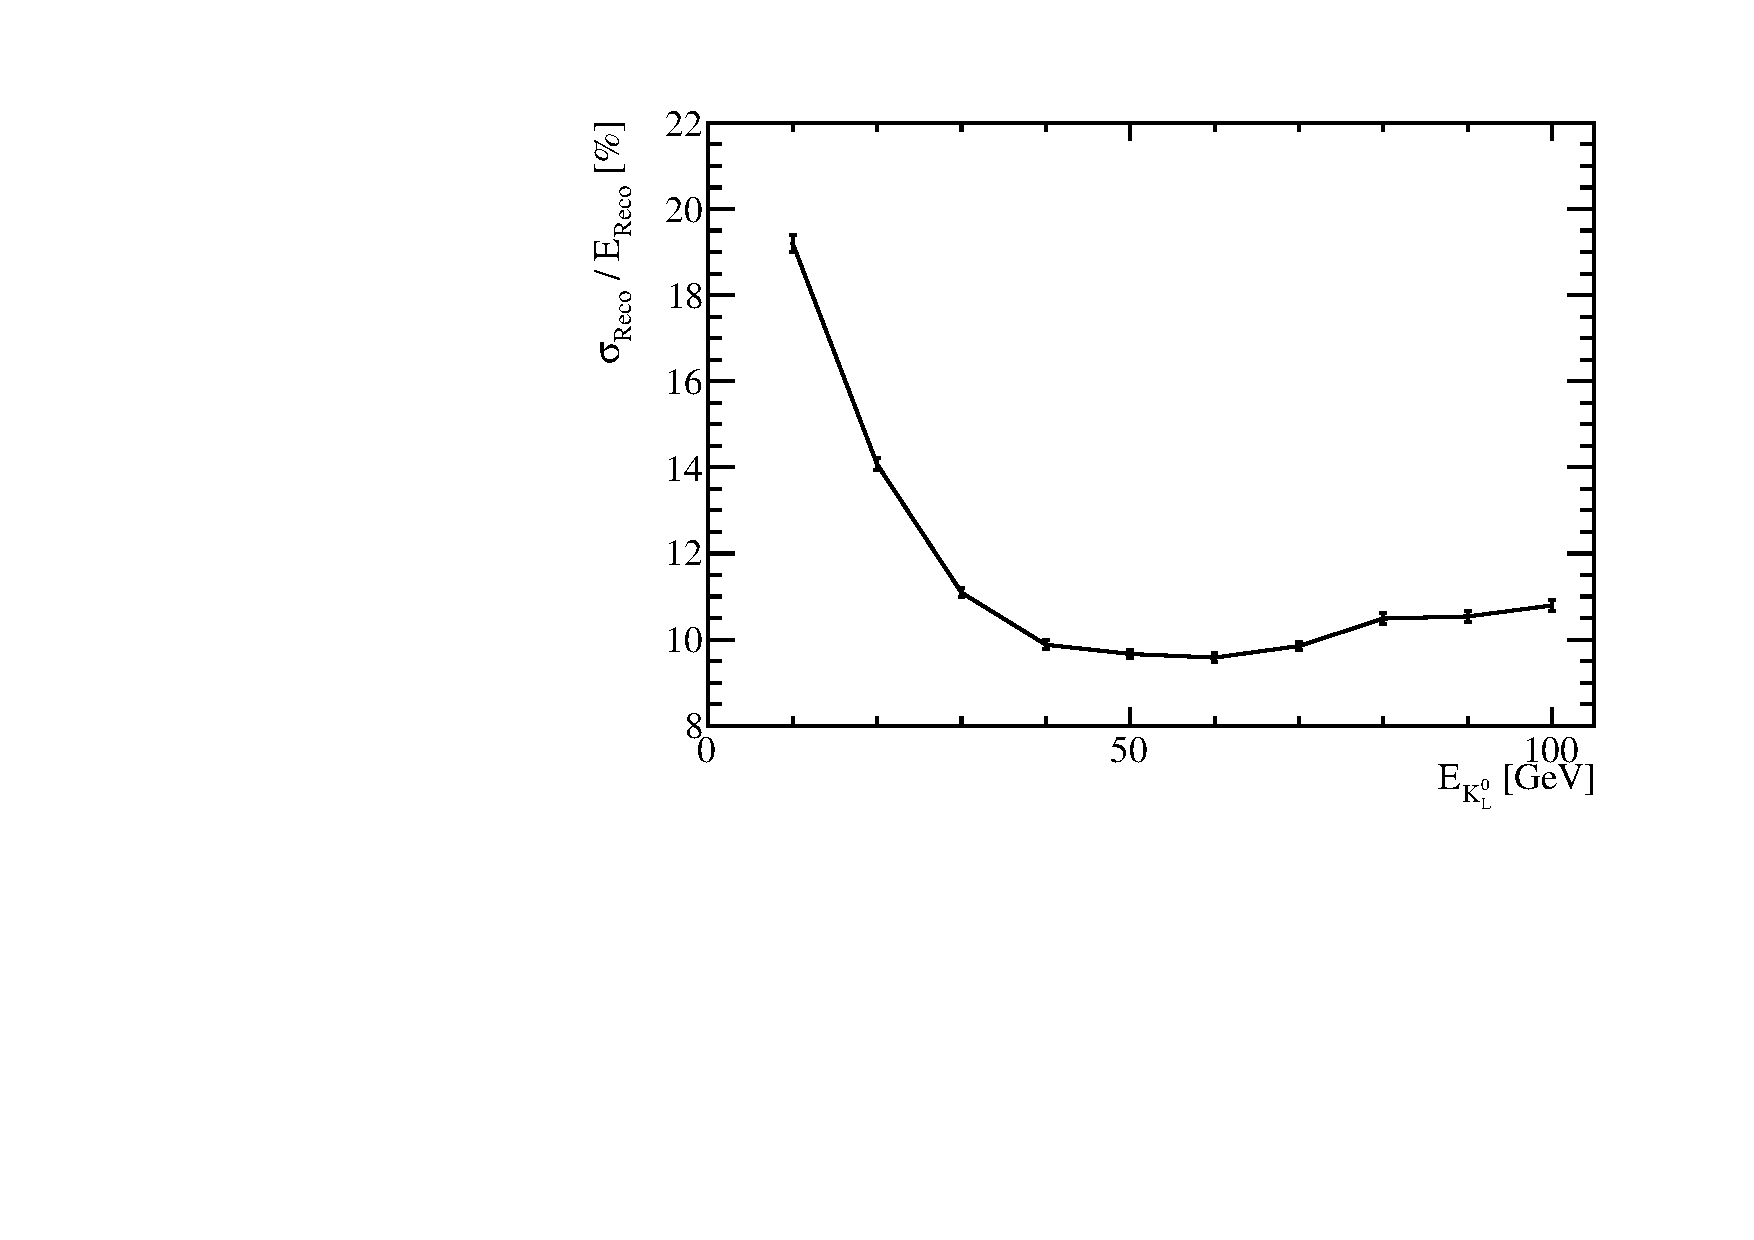
\includegraphics[width=0.5\textwidth]{OptimisationStudies/Plots/EnergyResolution/ER_vs_EKaon0L_SiECal.pdf}}
\subfloat[]{\label{fig:jernominalres}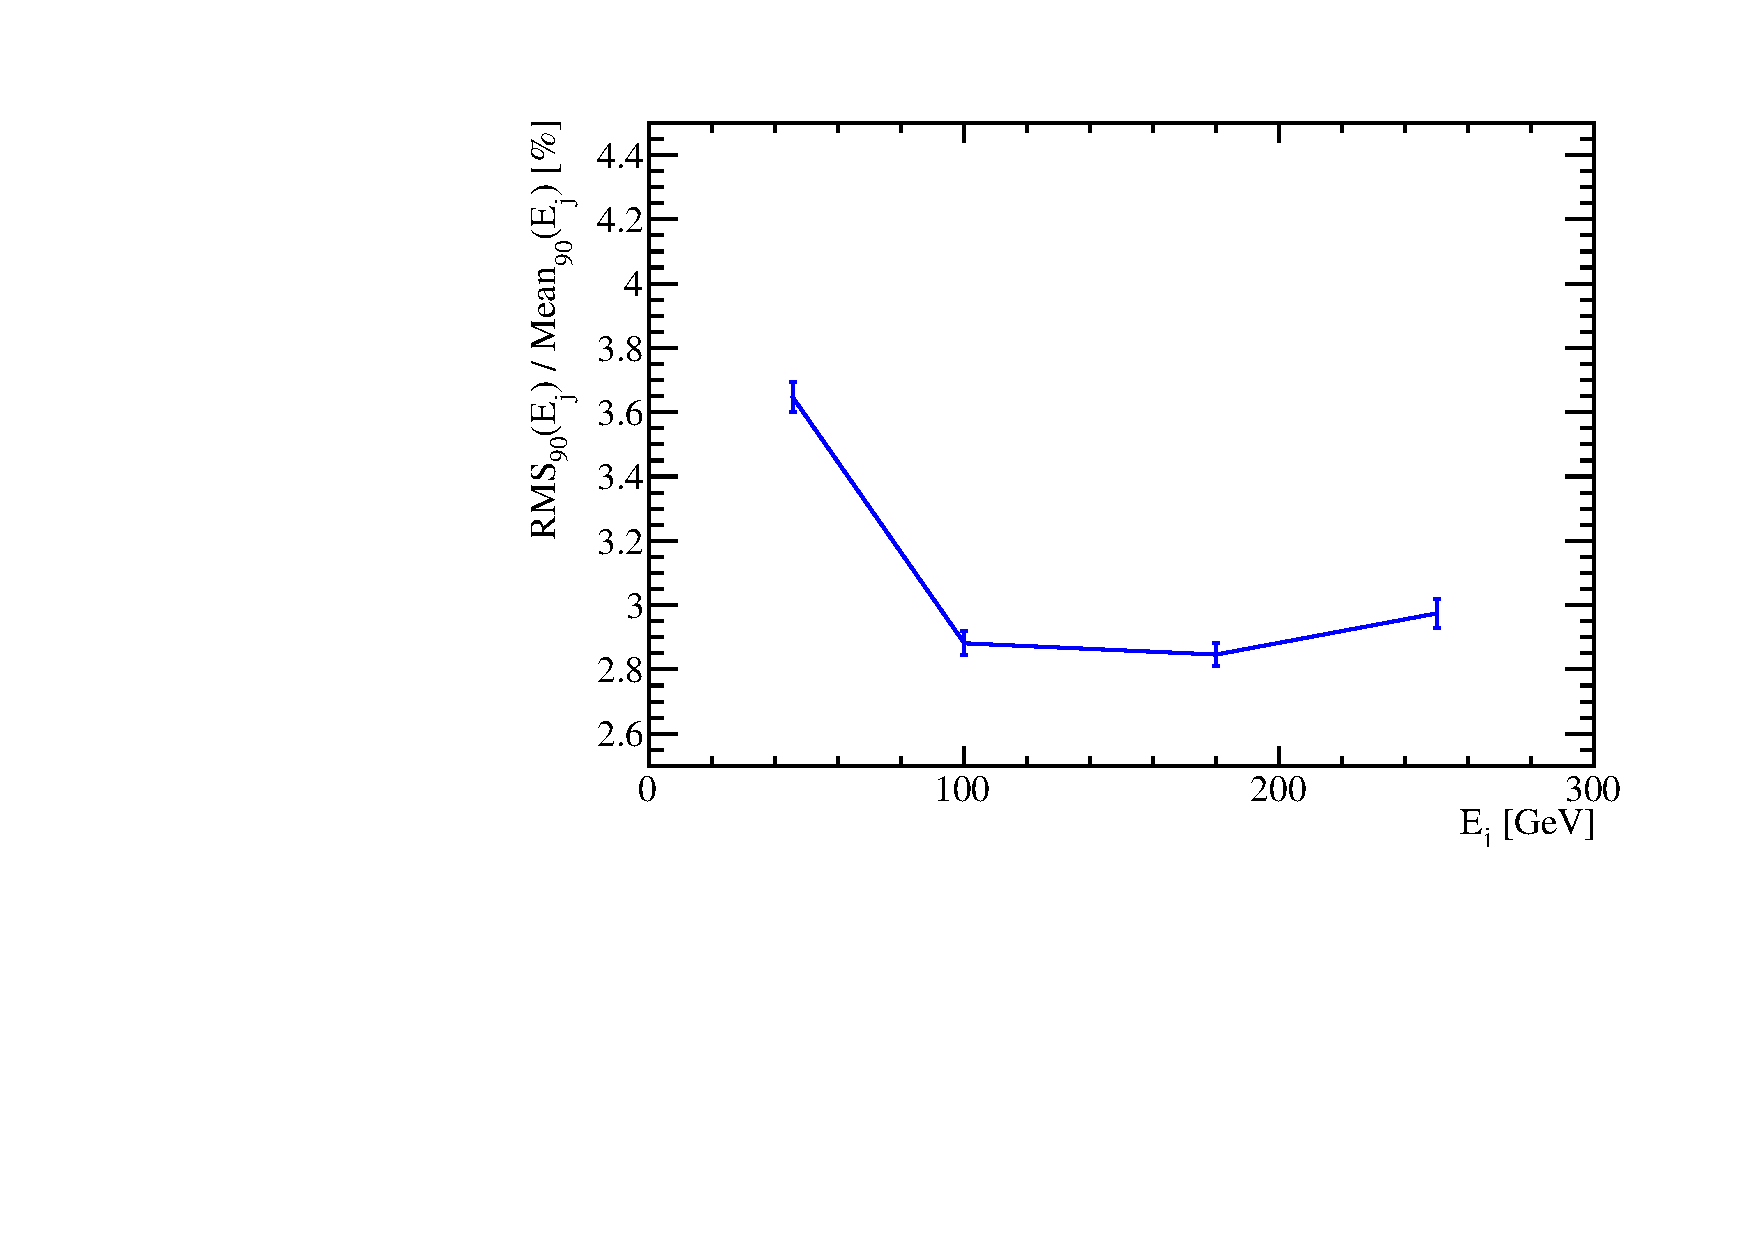
\includegraphics[width=0.5\textwidth]{OptimisationStudies/Plots/JetEnergyResolutions/JER_vs_JetEnergy_NominalDetectorPerformance.pdf}}
\caption[\protect\subref{fig:ecalsinominalres} The energy resolution as a function of photon energy for the silicon ECal option.  The black markers indicate the energy resolutions for the full ILD simulation.  \textcolor{blue}{The solid red line shows the test beam parameterisation of the ECal energy resolution and the blue shaded region indicates the uncertainty on the test beam parameterisation.} \protect\subref{fig:ecalscnominalres} The energy resolution as a function of photon energy for the scintillator ECal option.  The black markers indicate the energy resolutions for the full ILD simulation.  \textcolor{blue}{The solid red line shows the test beam parameterisation of the ECal energy resolution and the blue shaded region indicates the uncertainty on the test beam parameterisation.}  \protect\subref{fig:hcalnominalres} The energy resolution as a function of neutral hadron energy.  The black markers indicate the energy resolutions for the full ILD simulation, with the silicon ECal option, which was determined using $K^{0}_{L}$s.  The red solid line shows the test beam parameterisation of the HCal energy resolution, which was determined using $\pi^{\pm}$s.  \textcolor{blue}{The blue shaded region indicates the uncertainty on the test beam parameterisation.} \protect\subref{fig:jernominalres} The jet energy resolution ($\text{RMS}_{90}$) as a function of jet energy using the nominal ILD model, with the silicon ECal option.  The intrinsic energy resolution and confusion contributions these the jet energy resolutions are also presented.  The black dotted vertical line on the single particle energy resolutions shows the highest energy particles used in the test beam measurements.  The test beam parameterisation data was taken from \cite{Sefkow:2015hna}.]{\protect\subref{fig:ecalsinominalres} The energy resolution as a function of photon energy for the silicon ECal option.  The black markers indicate the energy resolutions for the full ILD simulation.  \textcolor{blue}{The solid red line shows the test beam parameterisation of the ECal energy resolution and the blue shaded region indicates the uncertainty on the test beam parameterisation.} \protect\subref{fig:ecalscnominalres} The energy resolution as a function of photon energy for the scintillator ECal option.  The black markers indicate the energy resolutions for the full ILD simulation.  \textcolor{blue}{The solid red line shows the test beam parameterisation of the ECal energy resolution and the blue shaded region indicates the uncertainty on the test beam parameterisation.}  \protect\subref{fig:hcalnominalres} The energy resolution as a function of neutral hadron energy.  The black markers indicate the energy resolutions for the full ILD simulation, with the silicon ECal option, which was determined using $K^{0}_{L}$s.  The red solid line shows the test beam parameterisation of the HCal energy resolution, which was determined using $\pi^{\pm}$s.  \textcolor{blue}{The blue shaded region indicates the uncertainty on the test beam parameterisation.} \protect\subref{fig:jernominalres} The jet energy resolution ($\text{RMS}_{90}$) as a function of jet energy using the nominal ILD model, with the silicon ECal option.  The intrinsic energy resolution and confusion contributions these the jet energy resolutions are also presented.  The black dotted vertical line on the single particle energy resolutions shows the highest energy particles used in the test beam measurements.  The test beam parameterisation data was taken from \cite{Sefkow:2015hna}.}
\label{fig:nominalres}
\end{figure}

%========================================================================================
%========================================================================================

